\documentclass[12pt, oneside, a4paper]{mwbk}
\usepackage[polish]{babel}
\usepackage[utf8]{inputenc}
\usepackage[OT4]{fontenc}

\usepackage{graphicx}
\usepackage{verbatim}

\usepackage[hidelinks]{hyperref}

\usepackage{titletoc}
\usepackage{etoolbox}

\usepackage{enumitem}
\usepackage[noend]{algorithmic}
\usepackage[polish,ruled]{algorithm2e}

\usepackage{color}
\usepackage[normalem]{ulem}

\usepackage{rotating}
\usepackage{float}
\usepackage{textpos}

\definecolor{dkgreen}{rgb}{0, 0.4, 0}


\linespread{1,3}
\oddsidemargin = 10pt
\textwidth = 470pt

\hyphenpenalty=1000
\tolerance=500

\setcounter{secnumdepth}{4}

\newcommand{\myfigure}[4]{\begin{figure}[H]
		\centering
		\scalebox{#3}
		{
			\includegraphics{#2}
		}
		\caption[#1]{#1}
		\label{#4}
	\end{figure}}
\usepackage{listings}
	
\lstset{frame=tb,
	aboveskip=3mm,
	belowskip=3mm,
	showstringspaces=false,
	columns=flexible,
	basicstyle={\small\ttfamily},
	numbers=none,
	numberstyle=\tiny\color{gray},
	keywordstyle=\color{blue},
	commentstyle=\color{dkgreen},
	stringstyle=\color{mauve},
	breaklines=true,
	breakatwhitespace=true,
	tabsize=3}
	
\newcommand{\beginnumbered}{\begin{enumerate}[label*=\arabic*.]}

\lstdefinelanguage{GLSL}
{
	sensitive=true,
	morekeywords=[1]{
		attribute, const, uniform, varying,
		layout, centroid, flat, smooth,
		noperspective, break, continue, do,
		for, while, switch, case, default, if,
		else, in, out, inout, float, int, void,
		bool, true, false, invariant, discard,
		return, mat2, mat3, mat4, mat2x2, mat2x3,
		mat2x4, mat3x2, mat3x3, mat3x4, mat4x2,
		mat4x3, mat4x4, vec2, vec3, vec4, ivec2,
		ivec3, ivec4, bvec2, bvec3, bvec4, uint,
		uvec2, uvec3, uvec4, lowp, mediump, highp,
		precision, sampler1D, sampler2D, sampler3D,
		samplerCube, sampler1DShadow,
		sampler2DShadow, samplerCubeShadow,
		sampler1DArray, sampler2DArray,
		sampler1DArrayShadow, sampler2DArrayShadow,
		isampler1D, isampler2D, isampler3D,
		isamplerCube, isampler1DArray,
		isampler2DArray, usampler1D, usampler2D,
		usampler3D, usamplerCube, usampler1DArray,
		usampler2DArray, sampler2DRect,
		sampler2DRectShadow, isampler2DRect,
		usampler2DRect, samplerBuffer,
		isamplerBuffer, usamplerBuffer, sampler2DMS,
		isampler2DMS, usampler2DMS,
		sampler2DMSArray, isampler2DMSArray,
		usampler2DMSArray, struct},
	morekeywords=[2]{
		radians,degrees,sin,cos,tan,asin,acos,atan,
		atan,sinh,cosh,tanh,asinh,acosh,atanh,pow,
		exp,log,exp2,log2,sqrt,inversesqrt,abs,sign,
		floor,trunc,round,roundEven,ceil,fract,mod,modf,
		min,max,clamp,mix,step,smoothstep,isnan,isinf,
		floatBitsToInt,floatBitsToUint,intBitsToFloat,
		uintBitsToFloat,length,distance,dot,cross,
		normalize,faceforward,reflect,refract,
		matrixCompMult,outerProduct,transpose,
		determinant,inverse,lessThan,lessThanEqual,
		greaterThan,greaterThanEqual,equal,notEqual,
		any,all,not,textureSize,texture,textureProj,
		textureLod,textureOffset,texelFetch,
		texelFetchOffset,textureProjOffset,
		textureLodOffset,textureProjLod,
		textureProjLodOffset,textureGrad,
		textureGradOffset,textureProjGrad,
		textureProjGradOffset,texture1D,texture1DProj,
		texture1DProjLod,texture2D,texture2DProj,
		texture2DLod,texture2DProjLod,texture3D,
		texture3DProj,texture3DLod,texture3DProjLod,
		textureCube,textureCubeLod,shadow1D,shadow2D,
		shadow1DProj,shadow2DProj,shadow1DLod,
		shadow2DLod,shadow1DProjLod,shadow2DProjLod,
		dFdx,dFdy,fwidth,noise1,noise2,noise3,noise4,
		EmitVertex,EndPrimitive},
	morekeywords=[3]{
		gl_VertexID,gl_InstanceID,gl_Position,
		gl_PointSize,gl_ClipDistance,gl_PerVertex,
		gl_Layer,gl_ClipVertex,gl_FragCoord,
		gl_FrontFacing,gl_ClipDistance,gl_FragColor,
		gl_FragData,gl_MaxDrawBuffers,gl_FragDepth,
		gl_PointCoord,gl_PrimitiveID,
		gl_MaxVertexAttribs,gl_MaxVertexUniformComponents,
		gl_MaxVaryingFloats,gl_MaxVaryingComponents,
		gl_MaxVertexOutputComponents,
		gl_MaxGeometryInputComponents,
		gl_MaxGeometryOutputComponents,
		gl_MaxFragmentInputComponents,
		gl_MaxVertexTextureImageUnits,
		gl_MaxCombinedTextureImageUnits,
		gl_MaxTextureImageUnits,
		gl_MaxFragmentUniformComponents,
		gl_MaxDrawBuffers,gl_MaxClipDistances,
		gl_MaxGeometryTextureImageUnits,
		gl_MaxGeometryOutputVertices,
		gl_MaxGeometryOutputVertices,
		gl_MaxGeometryTotalOutputComponents,
		gl_MaxGeometryUniformComponents,
		gl_MaxGeometryVaryingComponents,gl_DepthRange},
	morecomment=[l]{//},
	morecomment=[s]{/*}{*/},
	morecomment=[l][keywordstyle4]{\#},
}


\begin{document}
\author{Marcin Wawrzonowski}
\title{Wykorzystanie GPU urządzeń mobilnych w~symulacji dynamiki tkanin}
\begin{titlepage}
\thispagestyle{empty}
\begin{textblock}{1}(-2.65,-1.65)

\includegraphics{figures/tytulowa_pusta_mgrinz.pdf}
\end{textblock}
\vspace{7.3cm}
\begin{center}
\fontfamily{ptm}
\selectfont
\Huge
Wykorzystanie GPU urządzeń mobilnych w~symulacji dynamiki tkanin
\end{center}
\begin{center}
\fontfamily{ptm}
\selectfont
Praca dyplomowa inżynierska
\end{center}
\vspace{7.9cm}
\begin{center}
\fontfamily{ptm}
\selectfont
\hspace{-1cm}
\begin{tabular}{l}
Wydział Fizyki Technicznej, Informatyki i Matematyki Stosowanej \\
Promotor: dr inż. Dominik Szajerman \\
Dyplomant: Marcin Wawrzonowski \\
Nr albumu: 180729
\end{tabular}
\end{center}
\vspace{-.5cm}
\begin{center}
\fontfamily{ptm}
\selectfont
\begin{textblock}{13}(0,0.4)
Łódź, 2016
\end{textblock}
\end{center}
\end{titlepage}

\tableofcontents

\chapter{Wprowadzenie}
\label{t:wprowadzenie}


	\section{Aktualny stan zagadnienia}
	\label{t:wprowadzenie:stan}
	
		\subsection{Opis zagadnienia}
		\label{t:wprowadzenie:stan:opis}
		
		\subsection{Zastosowania}
		\label{t:wprowadzenie:stan:zastosowania}
		
		\subsection{Problemy}
		\label{t:wprowadzenie:stan:problemy}
		
		
	\section{Cel pracy}
	\label{t:wprowadzenie:cel}
	
	
	\section{Zakres pracy}
	\label{t:wprowadzenie:zakres}
	
	
	\section{Streszczenie}
	\label{t:wprowadzenie:streszczenie}
\chapter{Algorytmy symulacji tkanin}
\label{t:teoria}


	\section{Analiza istniejących modeli symulacji tkanin}
	\label{t:teoria:analiza}
	
		\subsection{Model masy na sprężynie}
		\label{t:teoria:analiza:masa}		
			
			Pierwszym z~rozważanych w niniejszej pracy modeli symulacji tkanin jest model masy na sprężynie. Rysowana przez API graficzne tkanina jest w postaci siatki wielokątowej. Siatka taka składa się z~punktów w przestrzeni 3D -- wierzchołków. Na potrzeby symulacji przyjęto, że każdy z~tych wierzchołków ma określoną masę i~poddano go działaniu sił, w wyniku których następuje przemieszczenie. Aby zachować kształt i~odpowiednie dla tkaniny zachowanie się siatki, wierzchołki połączone są sprężynami o~określonych współczynnikach sprężystości oraz tłumienia drgań. 
			
			
			\myownfigure{Schemat modelu masy na sprężynie. Kolorami zaznaczono wszystkie sprężyny biorące udział w obliczeniach położenia wierzchołka A.}{figures/pic_2_1.png}{0.22}{pic_2_1}
			
			
			Rysunek \ref{pic_2_1} przedstawia przykładowy fragment tkaniny opartej o~model masy na sprężynie. Założono dla uproszczenia, iż poszczególne wierzchołki tworzą kształt prostokątów, aczkolwiek w praktyce mogą przyjmować dowolne ustawienia. Ważne jednak dla zachowania poprawnej symulacji jest to, by punkty masy były równomiernie rozłożone na całej powierzchni tkaniny. W omawianym przypadku tak właśnie jest. 
			
			Można zaobserwować trzy rodzaje sprężyn, jakie występują w modelu na rysunku 2.1. Kolorem czerwonym zostały oznaczone sprężyny strukturalne, które służą do utrzymania ogólnego kształtu tkaniny. Jednakże one same nie są w stanie zasymulować zachowania tkaniny w~poprawny fizycznie i~wizualnie sposób. Kolorem zielonym narysowane zostały sprężyny odpowiedzialne za wierne oddanie zgięć tkaniny, położone są one wzdłuż diagonalnych krawędzi siatki. Kolorem niebieskim zaznaczono sprężyny, których obecność zapewnia tkaninie odpowiednią elastyczność i~chroni przed nadmiernym jej rozciąganiem. Łączą one nie sąsiednie wierzchołki, lecz następne za sąsiadem, w~tym samym kierunku. Każdy z~rodzajów sprężyn może być opisany innymi współczynnikami sprężystości i~tłumienia drgań, co pozwala na uzyskanie innych zachowań tkaniny w~symulacji.
			
			
			\myownfigure{Siły działające na pojedynczy wierzchołek.}{figures/pic_2_2.png}{0.3}{pic_2_2}
			
			
			Na rysunku \ref{pic_2_2} widać, jakie siły oddziałują na każdy punkt masy -- wierzchołek siatki tkaniny. Siły można zaklasyfikować jako wewnętrzne i zewnętrzne. Z~zewnętrznych wyróżniono siłę grawitacji, opisaną wzorem \cite{cloth-dobre-wzory}:
			
			\begin{equation}
			\mathbf{F_{g}} = m_{i} \cdot \mathbf{g} \ .
			\end{equation}
			
			Kolejna siła zewnętrzna to siła oporu powietrza. Zgodnie z Prawem Stokesa jest ona proporcjonalna do prędkości punktu masy oraz pewnego współczynnika oporu \emph{k} \cite{cloth-dobre-wzory}:
			
			\begin{equation}
			\mathbf{F_{a}} = -k_{a} \cdot \mathbf{v_{i}} \ .
			\end{equation}
			
			Siłami wewnętrznymi działającymi na wierzchołki tkaniny są oczywiście siły sprężystości, wynikające z istnienia omówionych wyżej sprężyn. Do wyznaczenia jej wartości wykorzystuje się Prawo Hooke'a, mówiące, że siła sprężystości oraz jej kierunek i~zwrot są proporcjonalne do wychylenia sprężyny, tj. różnicy odległości między jej aktualną długością, a~długością w~stanie spoczynku \cite{cloth-dobre-wzory}:
			
			\begin{equation}
			\mathbf{F_{se}} = - \sum_{n = 0}^{n < 12} k_{s} (|\mathbf{x_{i}} - \mathbf{x_{j}}| - l_{(i, j)}) \cdot \frac{\mathbf{x_{i}} - \mathbf{x_{j}}}{|\mathbf{x_{i}} - \mathbf{x_{j}}|} \ ,
			\end{equation}
			
			gdzie \(k_{s}\) -- współczynnik sprężystości, \(\mathbf{x_{i}}\) oraz \(\mathbf{x_{j}}\) -- położenia wierzchołków połączonych daną sprężyną, \(l_{(i, j)}\) -- odległość między tymi punktami w~stanie spoczynku.
			
			Zgodnie z \cite{receptury}, wprowadzono także siłę tłumienia drgań sprężystych, aby zminimalizować niepotrzebne, nierealistyczne drgania oraz ryzyko wymknięcia się symulacji spod kontroli. Nazywa się to ,,wybuchnięciem'' -- obliczane siły są takie, że pozycje wierzchołków dążą do nieskończoności. Tłumienie przedstawia się następującym wzorem:
			
			\begin{equation}
			\mathbf{F_{sd}} = \sum_{n = 0}^{n < 12} k_{d} (\frac{|\mathbf{x_{i}} - \mathbf{x_{j}}| \cdot |\mathbf{v_{i}} - \mathbf{v_{j}}|}{l_{(i, j)}}) \ ,
			\end{equation}
			
			gdzie oznaczenia są takie same, jak wyżej z~tym, że \(k_{d}\) jest tutaj współczynnikiem tłumienia drgań, \(|\mathbf{v_{i}} - \mathbf{v_{j}}|\) oznacza różnicę prędkości obu wierzchołków, a~działanie \(|\mathbf{x_{i}} - \mathbf{x_{j}}| \cdot |\mathbf{v_{i}} - \mathbf{v_{j}}|\) to iloczyn skalarny wektora różnicy położenia i~wektora różnicy prędkości. Końcowa siła sprężystości jest sumą dwóch powyższych wzorów. Można zapisać ją w~postaci:
			
			\begin{equation}
			\mathbf{F_{s}} = \mathbf{F_{se}} + \mathbf{F_{sd}} \ ,
			\end{equation}
			\begin{equation}
			\mathbf{F_{s}} = \sum_{n = 0}^{n < 12} - k_{s} (|\mathbf{x_{i}} - \mathbf{x_{j}}| - l_{(i, j)}) \cdot \frac{\mathbf{x_{i}} - \mathbf{x_{j}}}{|\mathbf{x_{i}} - \mathbf{x_{j}}|} + k_{d}(\frac{|\mathbf{x_{i}} - \mathbf{x_{j}}| \cdot |\mathbf{v_{i}} - \mathbf{v_{j}}|}{l_{(i, j)}}) \ .
			\end{equation}
			
			W sumie dla każdego wierzchołka rozważono 12 sił sprężystości dla wszystkich przyłączonych do niego sprężyn, siłę grawitacji oraz oporu powietrza. Należy zauważyć, że nie uwzględniono tutaj reakcji na kolizje -- będą one rozwiązane w~późniejszej sekcji algorytmu. Wzór na siłę wypadkową działającą na pojedynczy wierzchołek tkaniny oraz wypadkowe przyspieszenie można zapisać w~postaci:
			
			\begin{equation}
			\mathbf{F} = \mathbf{F}{s} + \mathbf{F}{g} + \mathbf{F}{d}		
			\end{equation}
			
			\begin{equation}
			\mathbf{a}(t) = \frac{\mathbf{F}}{m_{i}}	
			\end{equation}
			
			W celu wyznaczenia zmiany położenia punktu masy w~danym kroku symulacji, posłużono się, zgodnie z \cite{cloth-dobre-wzory} i \cite{receptury}, całkowaniem Verleta, będącym jedną z~technik całkowania numerycznego nie wprost. Opisane jest ono wzorem:
			
			\begin{equation}
			\mathbf{x}(t + \delta t) = 2\mathbf{x}(t) - \mathbf{x}(t - \delta t) + \mathbf{a}(t) \delta t^{2} \ ,		
			\end{equation}
			
			gdzie \(\mathbf{a(t)}\) jest przyspieszeniem, a~\(\mathbf{x}(t + \delta t)\), \(\mathbf{x}(t)\) i \(\mathbf{x}(t - \delta t)\) oznaczają położenia wierzchołka w~następnym, obecnym oraz poprzednim kroku symulacji. 
			
			Całkowanie Verleta jest równie proste obliczeniowo i~implementacjyjnie, jak najzwyklejsza metoda Eulera, a~zapewnia dużo stabilniejsze zachowanie się symulacji i~minimalizację tendencji do ,,wybuchnięcia''. Niejawnie obliczona zostaje tutaj aktualna prędkość wierzchołka, co sprawia, że do symulatora trzeba dostarczyć nie tylko obecną pozycję każdego punktu masy, ale także położenie poprzednie. Zwiększa to koszt pamięciowy symulacji względem innych technik całkowania, lecz zapewnia bardzo szybkie obliczenia i~stabilne ich wyniki.
		
		\subsection{Model oparty na pozycji}
		\label{t:teoria:analiza:poz}
		
			Model oparty na pozycji i~model masy na sprężynie mają pewną część wspólną -- jest to obliczanie przesunięć wynikających z~sił grawitacji oraz oporu powietrza za pomocą całkowania Verleta. Także tkanina ma w tym modelu taką samą postać, jak i~w~poprzednim -- zbiór wierzchołków, połączonych krawędziami, tworzących prostokątne kształty. Podejście do symulacji ruchów wynikających ze struktury samej tkaniny jest jednak kompletnie odmienne. Ponadto zaznaczyć należy, że w niniejszej pracy została wykorzystana tylko część aktualnie omawianego modelu, bardziej szczegółowo opisanego w~\cite{posbased}. Prezentowane tu rozwiązanie nie bierze pod uwagę ograniczników zginania oraz całego systemu detekcji kolizji, zaproponowanego w~rozdziale 4 \cite{posbased}.
			
			Przesunięcia wynikające z~sił zewnętrznych działających na układ nazywamy tutaj przesunięciami przewidywanymi. Każdy wierzchołek tkaniny opisywany jest, oprócz, masy, pozycji i~prędkości, także przez zbiór tzw. ograniczników. Każdy z nich definiowany jest poprzez pewną funkcję \(C_{j} : R^{3n_{j}} \rightarrow R\), zestaw indeksów \(\{ i_{1}, \dots, i_{n_{j}}  \}, i_{k} \in [1, \dots, N] \) i~parametr sztywności \(k \in [0\dots1] \). Ogranicznik może być typu równości, co oznacza, że jego ograniczenie jest spełnione, kiedy \( C_{j}(x_{i_{1}}, \dots, x_{i_{n_{j}}} ) = 0 \). Może być także typu nierówności, i~spełnia je warunek \( C_{j}(x_{i_{1}}, \dots, x_{i_{n_{j}}} ) \geq 0 \). W omawianym przypadku będą rozważane tylko ograniczniki pierwszego typu. Kluczowym elementem jest oczywiście funkcja \(C_{j}\), która określa sposób, w~jaki przewidywana pozycja zostanie poprawiona, od czego ta poprawa zależy -- czyli w~efekcie zachowanie się tkaniny. Funkcja ta może być zupełnie inna, gdy obliczane są ograniczenia przesuwania, a~inna przy ograniczeniach zginania bądź kolizjach. Widać, że dzięki temu model ten charakteryzuje się pewną elastycznością, a~ograniczniki są narzędziem, przy pomocy którego można realizować wiele rozmaitych założeń dotyczących ruchu tkaniny. Przesunięcia wynikające z~nałożonych ograniczników są obliczane po kolei, następnie pozycja przewidywana jest poprawiana do takiej, która spełnia wszystkie warunki, równości bądź nierówności, dla funkcji \(C_{j}\) ograniczników. Proces ten autorzy \cite{posbased} nazywają projekcją. Pod uwagę brana jest także sztywność ogranicznika, czyli procent, w~jakim się go stosuje.
			
			\myownfigure{Schemat działania ograniczników między dwoma punktami masy.}{figures/pic_2_3.png}{0.3}{pic_2_3}
			
			Podstawowym typem ogranicznika jest ogranicznik rozciągania. To on definiuje ogólny kształt i~odpowiednie zachowanie tkaniny. Jego funkcja ma postać:
			
			\begin{equation}
			C(\mathbf{p_{1}}, \mathbf{p_{2}}) = |\mathbf{p_{1}} - \mathbf{p_{2}}| - d \ .		
			\end{equation}
			
			Gdzie \( \mathbf{p_{1}} \) i \( \mathbf{p_{2}} \) są pozycjami rozpatrywanych wierzchołków, a~\(d\) - początkową odległością między nimi. Na rysunku \ref{pic_2_3} widać efekt projekcji. W~\cite{posbased} wyprowadzone zostają wzory na jej obliczenie, na podstawie funkcji \( C_{j}(x_{i_{1}}, \dots, x_{i_{n_{j}}} ) \):
			
			\begin{equation}
			s = \frac{C_{j}(\mathbf{p_{i_{1}}}, \dots, \mathbf{p_{i_{n_{j}}}} )}{ \sum _{j} w_{j} | \nabla _{\mathbf{p_{j}}} C_{j}(\mathbf{p_{i_{1}}}, \dots, \mathbf{p_{i_{n_{j}}}} ) | ^{2} } \ ,		
			\end{equation}
			
			\begin{equation}
			\delta \mathbf{p_{i}} = -sw_{i} \nabla _{\mathbf{p_{i}}} C_{j}(\mathbf{p_{i_{1}}}, \dots, \mathbf{p_{i_{n_{j}}}} ) \ .
			\end{equation}
			
			Gdzie \(w_{i}\) jest odwrotnością masy wierzchołka tkaniny. Biorąc pod uwagę, iż przemieszczenie jest do niej wprost proporcjonalne, można łatwo wyobrazić sobie dowód na poprawność tego podejścia -- w~przypadku, gdy masa cząstki jest nieskończona, przesunięcie będzie równe zeru. Kiedy na miejsce funkcji \(C_{j}(x_{i_{1}}, \dots, x_{i_{n_{j}}} ) \) wstawi się \(C(\mathbf{p_{1}}, \mathbf{p_{2}}) = |\mathbf{p_{1}} - \mathbf{p_{2}}| - d\), otrzymane zostaną po przekształceniach następujące wzory: 
			
			\begin{equation}
			\delta \mathbf{p_{1}} = - \frac{w_{1}}{w_{1} + w{2}} (|\mathbf{p_{1}} - \mathbf{p_{2}}| - d) \frac{\mathbf{p_{1}} - \mathbf{p_{2}}}{|\mathbf{p_{1}} - \mathbf{p_{2}}|} \ ,
			\end{equation}
			
			\begin{equation}
			\delta \mathbf{p_{2}} = \frac{w_{2}}{w_{1} + w{2}} (|\mathbf{p_{1}} - \mathbf{p_{2}}| - d) \frac{\mathbf{p_{1}} - \mathbf{p_{2}}}{|\mathbf{p_{1}} - \mathbf{p_{2}}|} \ .
			\end{equation}
			
			Da się zauważyć, że wzory (2.13) i (2.14) są bardzo podobne do wzoru (2.3). Tak samo, jak w modelu masy na sprężynie, ,,siła'' ogranicznika zależy od różnicy aktualnej odległości pomiędzy punktami masy i~odległości spoczynkowej. Rolę współczynnika sprężystości pełni tutaj parametr sztywności, przez który pomnożono na koniec przesunięcie będące wynikiem projekcji. Dla \(k\) równego 0 ogranicznik nie będzie w ogóle brany pod uwagę, a~dla równego 1 -- punkt nigdy nie zmieni swojej początkowej pozycji.
			
			W rozważanym przypadku nie zastosowano ograniczników zginania, użyto także innej metody detekcji kolizji. Autorzy \cite{posbased} używają ograniczników rozciągania biorąc pod uwagę tylko wierzchołki leżące w~sąsiedztwie danego punktu. Okazuje się, że podobny do użycia ograniczników zginania efekt można osiągnąć zwiększając zbiór rozpatrywanych wierzchołków o~te leżące jedną pozycję w siatce dalej - tak jak sprężyny oznaczone kolorem niebieskim na rysunku \ref{pic_2_1}. Przykładowo, ograniczając elastyczność przemieszczania wierzchołka \(A\) względem \(C\) ograniczamy przecież tak naprawdę możliwość zginania się trójkątów \(ABD\) i~\(BCD\) na wspólnej krawędzi \(BD\). Nie jest to tak dokładna metoda jak ograniczniki zginania, gdzie regulujemy kąt pomiędzy trójkątami, lecz mimo to daje ona poprawny wizualny efekt, jak pokazane zostanie w rozdziale 5. Jest też szybsza do obliczenia przez procesor, jako że sam wzór jest prostszy.
		
		\subsection{Porównanie powyższych metod}
		\label{t:teoria:analiza:porownanie}
		
			Podsumowując przedstawienie zastosowanych metod symulacji tkaniny, należy zauważyć, że każda z nich ma swoje plusy i~minusy. Największą zaletą modelu masy na sprężynie jest z pewnością prostota i~łatwość implementacji. Nietrudno wyobrazić sobie tkaninę, jako zbiór wierzchołków połączonych elastycznymi sprężynami, których siły sprężystości są wyliczane przy pomocy prostych praw fizyki. Trochę gorzej jest w przypadku drugiej omawianej metody -- tutaj zrozumienie zasady działania modelu wymaga wgłębienia się w wyprowadzenia wzorów matematycznych. Jednakże sama implementacja okazuje się równie prosta, ilość kodu jaką programista musi napisać, jest tak naprawdę podobna.
			
			Z pewnością największą zaletą modelu opartego na pozycji jest przewaga wydajnościowa. Wynika ona z~braku konieczności użycia całkowania numerycznego. Zachowanie tkaniny nie jest określane przez zbiór sił sprężystości, a~ograniczników, od razu modyfikujących pozycję. Całkować trzeba co najwyżej chcąc obliczyć siły zewnętrzne. Pozwala to na duże oszczędności obliczeniowe. W~przypadku modelu masy na sprężynie nie można uniknąć już tych obliczeń dla każdej ze sprężyn. W~celu uzyskania dokładniejszych wyników należy zastosować bardziej skomplikowane metody całkowania. Prowadzi to do spadku wydajności.
			
			Wyłania się tutaj także kolejna zaleta metody numer dwa. Numeryczne obliczanie przemieszczenia punktu masy wiąże się z~ryzykiem utraty stabilności symulacji i~jej ,,wybuchnięciem''. Przez większość czasu może ona pracować bezawaryjnie, dopóki nie zajdą pewne szczególne okoliczności, kiedy to wymyka się spod kontroli. Przykładem jest znaczna, skokowa zmiana parametru \( \delta t \) we wzorze (2.9) Doprowadzi ona do błędnego obliczenia wartości sił we wszystkich sprężynach -- będzie ona za duża, co z~kolei spowoduje niekontrolowane drgania, a~w~konsekwencji -- ,,wybuch''. W modelu opartym na pozycji korekcja przemieszczenia nie jest obliczana numerycznie i~gwarantuje to dużą stabilność działania tej metody.
			
			Jak widać, druga rozważana metoda wydaje się mieć przewagę nad pierwszą. Model oparty na pozycji daje nam bezpieczną i~wydajną obliczeniowo symulację, dlatego jest stosowany w wiodących na rynku, komercyjnych silnikach fizycznych. Jednakże model masy na sprężynie dużo łatwiej zrozumieć początkującemu programiście, a~do prostych zastosowań o~stałych parametrach nadaje się on równie dobrze.
		
		\subsection{Detekcja kolizji}
		\label{t:teoria:analiza:kolizje}
		
			Kluczowym aspektem symulacji tkaniny jest wykrywanie kolizji i~rozwiązywanie ich, czyli przemieszczanie wierzchołków tak, by obiekty się nie przenikały. Zwiększa to wrażenie autentyczności, realizmu symulacji z~punktu widzenia użytkownika. Do uzyskania odpowiedniego efektu musimy jednak zadbać także o~stabilność algorytmu rozwiązywania kolizji, chociażby po to, aby uniknąć znanego chyba wszystkim użytkownikom wirtualnych symulacji i~gier efektu ''podrygiwania''. Obliczenia mogą pochłonąć tu bardzo dużo czasu procesora, dlatego kluczowy jest dobór odpowiednio wydajnego algorytmu, szczególnie, że w niniejszej pracy rozważa się implementację symulacji na urządzeniu mobilnym. Dlatego właśnie w~tej kwestii uwagę poświęcono na najprostszym rozwiązaniom.
		
			\subsubsection{Kolizje zewnętrzne}
			\label{t:teoria:analiza:kolizje:zewn}
			
				Poprzez kolizje zewnętrzne rozumiemy kolizje wierzchołków tkaniny z~innymi obiektami sceny, np. podłogą pomieszczenia. Wykrywanie ich oraz generowanie odpowiedniej reakcji jest absolutnie niezbędne do zasymulowania jakiejkolwiek interakcji z resztą wirtualnego świata. W~tym celu zastosowano sfery okalające, zwane dalej BS od angielskiego \emph{Bounding Sphere} oraz prostopadłościany okalające, prostopadłe do osi układu współrzędnych, zwane dalej AABB od angielskiego \emph{Axis-Aligned Bounding Box}.\newpage
				
				\myownfigure{Przykład kolizji sfer okalających.}{figures/pic_2_4.png}{0.3}{pic_2_4}		%R1, R2, d
				
				Sfery okalające są najprostszą w implementacji i~najszybszą obliczeniowo metodą detekcji kolizji. Na rysunku \ref{pic_2_4} widać, jak wygląda przykładowy układ dwóch BS, oraz w~jaki sposób ustawiona może być BS względem obiektu. Wykrycie przecięcia się polega na porównaniu sumy długości promieni \(R_{1}\) i~\(R_{2}\) obu sfer z~odległością pomiędzy ich środkami \(d\). Jeżeli
				
				\begin{equation}
				R_{1} + R_{2} < d \ ,
				\end{equation}
				
				to znaczy, że doszło do kolizji i~sferę, która przemieszczając się, do niej doprowadziła, należy odpowiednio przesunąć tak, by się one nie przecinały. Mowa tutaj o~tzw. rozwiązaniu kolizji. Dokonano tego w prosty sposób \cite{wzory_sfera}:
				
				\begin{equation}
				\mathbf{p}_{i} = \mathbf{p}_{i} + (\frac{\mathbf{p}_{C1} - \mathbf{p}_{C2}}{|\mathbf{p}_{C1} - \mathbf{p}_{C2}|})(R_{1} + R_{2} - d) \ .
				\end{equation}
				
				Jak można się domyślić, wadą sfer okalających jest ich niska dokładność -- obiekty idealnie kuliste rzadko występują w~świecie rzeczywistym. Na potrzeby symulowania świata otaczającego tkaninę w niniejszej pracy jednak takie rozwiązanie w~zupełności wystarcza. Przyjęto, że każdy wierzchołek posiada swoją własną BS, o~pozycji środka identycznej z pozycją punktu oraz o~promieniu równym pewnemu procentowi najkrótszej odległości między dwoma wierzchołkami, mniejszemu niż jej połowa. W każdym kroku symulacji każdy z~nich zostaje sprawdzony, czy nie zaszła kolizja z którymś, bądź wieloma, obiektami sceny. Jeśli tak, poprawia się jego położenie. 
				
				Jest to rozwiązanie szybkie, jednak ma jedną istotną wadę - BS nie pokrywają całej powierzchni siatki tkaniny, a tylko obszary w okolicach wierzchołków. Kolizje na środkach trójkątów nie są sprawdzane, co może doprowadzić do przenikania obiektów przez tkaninę przy niskiej jej rozdzielczości. Założono jednak, że jest to rozwiązanie wystarczające -- nie obciążamy urządzenia mobilnego nadmiarem obliczeń związanych z detekcją kolizji. Poza tym gęstość siatki potrzebna do odwzorowania realistycznego wyglądu tkaniny jest na tyle duża, by szczeliny pomiędzy BS były na tyle małe, aby sensownie zminimalizować ryzyko wystąpienia przenikania.
				
				\myownfigure{Przykład kolizji BS z prostopadłościanem AABB.}{figures/pic_2_5.png}{0.3}{pic_2_5}		%dwa boksy p1min, p1max, p2min, p2max
				
				Obiekty zewnętrzne znajdujące się w świecie symulacji mogą posiadać dwa rodzaje detektorów kolizji. Są albo sferami okalającymi, w którym to przypadku do wykrycia przecięć zastosowane zostają opisane powyżej wzory (2.15) i (2.16), albo AABB -- prostopadłościany, których położenie i~rozmiary są wyznaczane przez dwa punkty w przestrzeni: minimum \(\mathbf{p}_{i_{min}}\) oraz maksimum \(\mathbf{p}_{i_{max}}\). W jaki sposób figury są tworzone na podstawie tych dwóch pozycji -- widać na rysunku \ref{pic_2_5}. Można zauważyć, że ten sposób interpretacji dwóch wymienionych wyżej danych skutkuje niską zajętością pamięciową (tylko dwa wektory trójwymiarowe reprezentują AABB) oraz prostotą wzorów wykrycia przecięcia, a~co za tym idzie -- szybkością obliczeń tychże. Ewidentną wadą jest jednak znowu niska dokładność -- fakt, że kolejne ścianki prostopadłościanu zawsze będą prostopadłe do kolejnych osi układu współrzędnych. Utrudnia to odwzorowanie dokładnych kolizji np. dla obiektów pochyłych. Detekcja i~rozwiązanie przecięć pomiędzy AABB i BS następuje według nieco innych zasad, niż w~przypadku dwóch BS \cite{wzory_sfera} \cite{wzory_sfera_box}:
				
				\begin{equation}
				\mathbf{c}_{i} =  min(max(\mathbf{p}_{C1}, \mathbf{p}_{i_{min}}), \mathbf{p}_{i_{max}})  \ .
				\end{equation}
				
				\begin{equation}
				\mathbf{p}_{i} = \mathbf{p}_{i} + \frac{\mathbf{c}_{i}}{|\mathbf{c}_{i}|}(R1 - |\mathbf{c}_{i} - \mathbf{p}_{C1}|) \ .
				\end{equation}
			
			\subsubsection{Kolizje wewnętrzne}
			\label{t:teoria:analiza:kolizje:wewn}
			
				\myownfigure{Ułożenie sfer kolizyjnych w~wierzchołkach tkaniny.}{figures/pic_2_6.png}{0.4}{pic_2_6}		% schemat sfer kolizyjnych dla siatki
				
				Podczas bardziej dynamicznych i gwałtownych ruchów symulowanej siatki, może dochodzić do przenikania się przez siebie jej fragmentów. Rozwiązując kolizje wewnętrzne, postarano się wyeliminować ten niepożądany artefakt wizualny. Na rysunku \ref{pic_2_6} widać, jak wygląda mechanizm dla pojedynczego wierzchołka. W~sekcji \ref{t:teoria:analiza:kolizje:zewn} ustalono, że wszystkie punkty masy posiadają swoją własną sferę okalającą. Tutaj dalej z~tego faktu skorzystano, po prostu rozwiązując kolizje BS każdego wierzchołka z BS jego ośmiu sąsiadów położonych w najbliższym otoczeniu. Zapewnia to redukcję minimalnych przecięć w bezpośrednim sąsiedztwie punktów masy, które pojawiałyby się już przy swobodnym ruchu tkaniny, z~oddziałującymi tylko siłami grawitacji i~oporu powietrza.
				
				Zastosowany mechanizm z~oczywistych względów nie jest doskonały. Nie zabezpiecza przed przenikaniem się w sytuacji, gdy np. róg tkaniny przemieści się przez jej środek. Jednakże zarówno bardziej wyrafinowane metody detekcji przecięć, jak i~sprawdzanie kolizji BS -- BS na zasadzie ,,każdy z~każdym'' wiążą się z~bardzo dużym narzutem obliczeniowym, wielokrotnie większym niż przesuwanie wierzchołków będące efektem działania modelu symulacji. W związku z~tym na potrzeby niniejszej pracy została użyta bardzo prosta, acz niedoskonała, opisana powyżej technika. Biorąc pod uwagę, iż tkanina zawieszona jest na stałe za dwa, nie poruszające się, górne narożniki, prawdopodobieństwo wystąpienia przecięcia nie jest duże. Założono więc, że sprawdzanie kolizji tylko w najbliższym otoczeniu każdego z~wierzchołków okaże się wystarczające wizualnie.
			
	\section{Obliczenia GPGPU a symulacja tkanin}
	\label{t:teoria:gpu}
	
		\subsection{Definicja GPGPU}
		\label{t:teoria:gpu:gpgpu}
		
		Pierwsze układy GPU -- \emph{Graphics Processing Unit} -- zwane też kartami graficznymi, pojawiły się już w~latach siedemdziesiątych XX wieku \cite{gpu_wiki}. Od początku były to wyspecjalizowane urządzenia peryferyjne służące do wyświetlania grafiki, początkowo 2D, później, w miarę ewolucji, 3D. Przez bardzo długi czas pracowały one w~układzie zamkniętym -- programista dostarczał tylko określone dane, potrzebne do narysowania obiektu, np. bufory pozycji i~indeksów wierzchołków, a GPU rysowało je w~taki sposób, w~jaki zostało zaprogramowane w~fabryce. Twórca gry bądź wizualizacji graficznej, nie miał kompletnie wpływu na przebieg procesu rysowania, ani na to, jakie dokładnie obliczenia zostaną wykonane. 
		
		Zmieniło się to na początku XXI wieku, wraz z~premierą układu NVIDIA GeForce 3 \cite{gpu_wiki}. Wprowadził on otwarty, programowalny potok renderingu. Pisząc tzw. vertex i~pixel shadery, programista od tego momentu mógł kontrolować sposób, w~jaki rysowanie przebiegało, mając możliwość ulepszenia starych, wysłużonych technik. 
		
		Chcąc sprostać zapotrzebowaniu na coraz to bardziej realistyczną grafikę, producenci z~biegiem lat szybko zwiększali moc obliczeniową kart graficznych. Były one jednak cały czas urządzeniami przeznaczonymi ściśle do generowania grafiki. Aby wykorzystać ich potęgę do innych celów niż rendering, należało dopasować pisane programy do API graficznego, co bardzo utrudniało proces ich powstawania. Dopiero wejście na rynek technologii takich, jak NVIDIA CUDA bądź OpenCL zapewniło dostęp do wszystkich funkcji GPU z~wykorzystaniem danej platformy, niezwiązanej z renderingiem i~niewymagającej jego znajomości. Obliczenia ogólnego przeznaczenia, najczęściej wykonywane za pomocą wymienionych wyżej API, nazywa się właśnie GPGPU -- \emph{General Purpose computing on~Graphics Processing Units}. Ogólnie można powiedzieć, że każdy język, czy technologia, która pozwala na pobranie wynikowych danych programu uruchamianego na GPU daje możliwość wykorzystania go do GPGPU \cite{gpu_wiki}. Mają one zastosowanie w wielu dziedzinach, chociażby w modelowaniu matematycznym, statystyce, medycynie bądź silnikach i~symulacjach fizycznych -- chociażby właśnie modelowania tkaniny. 
	
		\subsection{Architektura i programowanie GPU}
		\label{t:teoria:gpu:architektura}
		
		\myownextfigure{Typowa architektura GPU.}{figures/pic_2_7.png}{0.3}{pic_2_7}		% schemat GPU
		% kiedy i po co GPU, dzisiejsze zastosowania, GPGPU, równoległość obliczeń, podział na SM, SP, wątki, dzisiejsze wydajności
		
		\footnotetext{https://goo.gl/VEjIeU}
		GPU jest układem złożonym z~wielu jednostek obliczeniowych, pracujących ze sobą równolegle. Zrównoleglenie obliczeń wynika z~charakterystyki pierwotnego zastosowania GPU, czyli renderingu grafiki. Obliczenia na każdym wierzchołku, bądź fragmencie obrazu są zazwyczaj niezależne od siebie i~takie same dla każdego z nich. Można więc dla tychże elementów identyczny ciąg instrukcji wykonywać równolegle, dostarczając do niego inne dane. GPU jest sztandarowym przykładem wdrożenia architektury SIMD (\emph{Single Instruction, Multiple Data} \cite{simd}). Jak się szybko okazało, ten model przetwarzania znalazł zastosowanie nie tylko przy rysowaniu trójkątów, ale też w~wielu innych dziedzinach, często niezwiązanych z~grami czy wizualizacjami.
		
		Na rysunku \ref{pic_2_7} widać budowę przykładowego układu, jednakową dla większości tego typu urządzeń. Nadrzędną jednostką, z której składa się GPU jest multiprocesor strumieniowy (SM -- \emph{Streaming Multiprocessor}), będący samodzielną jednostką obliczeniową, aczkolwiek dzielący część pamięci z~innymi SM. Przykładowo karta grafiki NVIDIA GeForce 9800 GTX ma osiem SM. Każdy z nich dzieli się na procesory strumieniowe (SP -- \emph{Streaming Processor}), w~danym przypadku jest ich w sumie 128 na całym GPU. SP są tak skonstruowane, by móc przetwarzać jak najwięcej operacji równolegle. W technologiach stricte GPGPU programista zależnie od potrzeb może uruchomić konkretną liczbę SP, na każdym zaprzęgając do pracy ustaloną z~góry liczbę wątków, nieprzekraczającą jednak maksymalnej wartości, zależnej od modelu urządzenia \cite{cuda}.
		
		\myextcitefigure{Schemat tzw. gridu w technologii CUDA}{\cite{cuda}.}{figures/pic_2_8.png}{0.45}{pic_2_8}		% schemat gridu CUDA'owego
		
		Jednakże zazwyczaj nie ma bezpośredniej kontroli nad elementami warstwy fizycznej wymienionymi wyżej. Przykładowo, CUDA zapewnia programiście warstwę logiczną podziału na jednostki przetwarzające (zwane tu blokami) i~wątkami. Widać to na rysunku \ref{pic_2_8}. W przypadku OpenCL sytuacja wygląda podobnie. Programista może oznaczyć, jak chce podzielić zadania, jednak przypisanie ich do konkretnych procesorów leży już w gestii samego API i~sterownika. Na GPU stworzonym w architekturze Fermi istnieje możliwość zdefiniowania w sumie \(65\ 535 \times 65\ 535 \times 1536\) wątków pracujących współbieżnie \cite{cuda}.\newpage
		
		\myownfigure{Potok renderingu i transformacyjne sprzężenie zwrotne.}{figures/pic_2_9.png}{0.3}{pic_2_9}		% jak to działa w api graficznym
		
		Chcąc korzystać z~API graficznego do obliczeń GPGPU, programista zostaje skazany na pisanie programów w~natywnym języku shaderów, najczęściej HLSL (dla API DirectX) lub GLSL (dla API OpenGL). Te wysokopoziomowe są bardzo podobne do zwykłego C, więc opanowanie ich nie powinno nastręczać problemów, jednakże wymagają wiedzy na temat przebiegu procesu renderingu. Kontrola nad przydziałem i~liczbą jednostek przetwarzających także wygląda w inaczej. Jedyną możliwością jej zdefiniowania jest ustalenie danej, konkretnej liczby wierzchołków przesyłanych w~buforze do GPU, które, w zależności od potrzeb, mogą być z~logicznego punktu widzenia faktycznymi wierzchołkami, bądź po prostu zbiorami danych o~z~góry ustalonej strukturze. Rysunek 2.9 obrazuje proces przetwarzania danych zaszytych w wierzchołkach. Twórcy API graficznych od pewnego momentu starają się także umożliwić i~ułatwić obliczenia GPGPU za ich pomocą, udostępniając takie funkcje, jak np. transformacyjne sprzężenie zwrotne, czy bufory teksturowe w OpenGL \cite{receptury}. \newpage
		
		\subsection{Porównanie GPU i CPU pod kątem architektury i zastosowań}
		\label{t:teoria:gpu:porownanie}
		
		\myownextfigure{Porównanie budowy CPU i GPU.}{figures/pic_2_10.png}{0.3}{pic_2_10}		% proste schematy GPU i CPU obok
		\footnotetext{http://blog.goldenhelix.com/mthiesen/video-graphics-and-genomics-a-real-game-changer/}
		
		Rysunek \ref{pic_2_10} przedstawia uproszczone schematy architektury CPU i~GPU, co doskonale obrazuje różnice między nimi, a~także pozwala wywnioskować zastosowania. W~rozdziale \ref{t:teoria:gpu:architektura} podano, że GPU jest urządzeniem zbudowanym z~wielu procesorów pracujących równolegle, natomiast CPU składa się z~niewielkiej liczby jednostek obliczeniowych (w~dzisiejszych czasach 4~to standardowa liczba dla zapotrzebowań osobistych), jednakże dużo szybszych. Procesory CPU są dużo bardziej zaawansowane technologiczne, wyposażone w~większą liczbę zaawansowanych instrukcji oraz algorytmów przyspieszających ich działanie w~specjalnych sytuacjach. Przykładem może być predykcja wyboru instrukcji warunkowych, znacznie skracająca czas obliczeń bloków \texttt{if-else} \cite{branch_prediction_wiki}. Z kolei w~GPU ta technologia jest dużo uboższa. Wynika z tego, że sekwencyjny kod z~dużą liczbą rozgałęzień szybciej działa na CPU, a~GPU nadaje się lepiej do obliczeń równoległych, w~których warunków należy unikać. 
		
		\myextfigure{Różnica rozwoju wydajności CPU i GPU na przestrzeni ostatnich lat.}{figures/pic_2_11.png}{0.5}{pic_2_11}		% 2 wykresy - przewaga GPU nad CPU w danych obliczeniach i odwrotnie
		\footnotetext{https://algconsultings.wordpress.com/2011/02/28/can-we-afford-to-have-a-supercomputer}
		
		Na rysunku \ref{pic_2_11} widać, że na przestrzeni ostatnich lat teoretyczna wydajność kart graficznych, liczona w gigaflopach na sekundę, wzrosła znacznie w~stosunku do procesorów. Można zaobserwować kolejny rozstrzał między tymi platformami, CPU nie robi większej różnicy precyzja liczb, na których wykonywane jest przetwarzanie. Natomiast GPU zoptymalizowana jest pod kątem obliczeń na zmiennych typu \texttt{float} -- pojedynczej precyzji. Prawdopodobnie po raz kolejny widać skutki najczęstszego stosowania GPU do renderingu grafiki trójwymiarowej, gdzie pojedyncza precyzja jest wystarczająca.
		
		CPU zapewnia także dużo potężniejszy i~bardziej złożony system komunikacji między pracującymi wątkami oraz większą liczbę struktur synchronizacyjnych. W przypadku GPU synchronizacja opiera się głównie o~bariery pamięciowe, pozwalające wstrzymać wątki, dopóki inne nie dotrą do tego samego miejsca kodu, jednakże tylko w ograniczonym zakresie, np. na poziomie bloku, oraz o operacje atomowe \cite{cuda}. Trudno uzyskać także specjalizację wątków do określonych zadań, jako, że ten sam program, zwany \emph{kernelem}, jest uruchamiany na nich wszystkich w~jednym momencie. To, nad czym programista ma kontrolę, to ich liczba oraz początkowy zbiór danych.
		
		Największym problemem CPU jest to, że osiągnęły one szczyt swoich możliwości w~kwestii szybkości taktowania zegara. Nie jest możliwe dalsze jej zwiększanie bez gwałtownego wzrostu ilości produkowanego ciepła. Wymaga to zaawansowanych rozwiązań chłodzących i~dla zwykłego zjadacza chleba staje się nieosiągalne finansowo. W kontraście, procesory GPU cały czas pracują z~relatywnie niskimi częstotliwościami, a~ich rozwój polega w skrócie na dokładaniu kolejnych jednostek przetwarzających i~zmniejszaniu zapotrzebowania na energię.
		
		\subsection{Zastosowanie GPU w symulacji tkanin}
		\label{t:teoria:gpu:zalety}
		
		Siłą rzeczy narzuca się pytanie, zadane w~kontekście niniejszej pracy -- co lepiej nadaje się do obliczeń związanych z~symulacją tkaniny? CPU czy GPU? Odpowiedź zdaje się być w~miarę oczywista. Rozważany układ jest zbiorem wierzchołków, do których przyłączona jest pewna z~góry określona ilość sprężyn bądź ograniczników. Każdy z~nich jest oddzielnym bytem i~dla każdego wykonujemy tak naprawdę te same obliczenia (tzn. ten sam ciąg instrukcji). Sensownym pomysłem w takiej sytuacji wydaje się przeprowadzenie ich równolegle. 
		
		Można podejść do tego na dwa sposoby. Pierwszym jest przyjęcie punktu masy tkaniny jako ,,jednostki obliczeniowej'' i~rozwiązanie sił bądź przesunięć dla każdej z przyłączonych do niego sprężyn. Jak jednak widać na rysunku \ref{pic_2_1}, wierzchołki współdzielą sprężyny, tzn. wartość siły dla AB będzie taka sama jak dla BA, tylko nada się jej przeciwny zwrot. Przedstawione powyżej podejście doprowadzi do redundancji obliczeń. Drugi sposób zakłada policzenie wpierw sił dla wszystkich sprężyn, a~następnie dopiero zmodyfikowanie pozycji wierzchołków na ich podstawie. Wadą tego rozwiązania jest konieczność uruchamiania dwóch różnych programów na GPU i~spowolnienie programu poprzez nieuchronny powrót sterowania do CPU pomiędzy obliczeniami, ewentualnie konieczność synchronizacji dostępu do danej komórki pamięci przechowującej pozycję danego wierzchołka, jako, że jedna sprężyna wpływa na dwa punkty masy. W związku z~tym w niniejszej pracy zdecydowano się na metodę pierwszą.
		
		W przypadku chęci stworzenia implementacji symulacji na CPU, należałoby sekwencyjnie wykonywać wszystkie obliczenia na kolejnych wierzchołkach, kolejno w pętli. W najlepszym przypadku można podzielić przetwarzanie na wątki, jednak maksymalnie i~tak byłoby dostępnych niewiele jednostek przetwarzających. W GPU jest ich dużo więcej, oprócz tego urządzenie z definicji przystosowano do obliczeń równoległych, co pozwala uzyskać maksymalną wydajność. Jedyną sytuacją, w której CPU mogłoby mieć przewagę, jest detekcja dużej liczby kolizji, z~racji konieczności użycia tutaj instrukcji warunkowych, a~jak wiemy, GPU nie najlepiej sobie z nimi radzi.
		
		\myextcitefigure{Porównanie wydajności implementacji CPU i GPU}{\cite{bibid}.}{figures/pic_2_12.png}{0.395}{pic_2_12}		% wykres - porównanie GPU i CPU dla tkanin
		
		Autorzy \cite{deformable} wykonali porównanie szybkości przetwarzania symulacji tkaniny osobno dla CPU i~GPU. Widać tutaj miażdżącą przewagę karty graficznej nad procesorem w~kwestii wydajności, co pozwala wnioskować o sensowności zastosowania GPU do rozwiązania omawianego problemu.

\chapter{Wykorzystane technologie}
\label{t:technologie}


	\section{Analiza możliwości urządzeń mobilnych}
	\label{t:technologie:mobilne}
	
		\subsection{Sensowność wykorzystania urządzeń mobilnych w symulacji tkanin}
		\label{t:technologie:mobilne:dlaczego}
	
		\subsection{Konfiguracja sprzętowa i możliwości}
		\label{t:technologie:mobilne:konfiguracja}
		
		\subsection{Porównanie wydajności i możliwości przykładowego komputera PC i smartfona}
		\label{t:technologie:mobilne:porownanie}

	
	\section{Przedstawienie wybranych technologii i narzędzi}
	\label{t:technologie:narzedzia}
	
		\subsection{OpenGL ES 3.0}
		\label{t:technologie:mobilne:ogl}
		
		\subsection{GLSL}
		\label{t:technologie:mobilne:glsl}
		
		\subsection{Android NDK}
		\label{t:technologie:mobilne:ndk}
		
		\subsection{Visual Studio 2015 Community + Cross-platform Development Kit}
		\label{t:technologie:mobilne:vs}
\chapter{Budowa i działanie aplikacji}
\label{t:praktyka}
	
	\section{Cele oraz możliwości aplikacji}
	\label{t:praktyka:cel}
	
	% co program ma robić
	
	Na potrzeby niniejszej pracy została stworzona aplikacja prezentująca. Jej działanie realizuje kilka kluczowych celów. Po pierwsze, ma ona za zadanie zaprezentować działanie dwóch omówionych w Rozdziale \ref{t:teoria} modeli symulacji tkanin. Musi pozwalać na porównanie ich pod względem wydajności, stabilności i efektu wizualnego. Wydajność rozumiemy poprzez czas potrzebny na obliczenie jednego kroku symulacji, im mniejszy, tym oczywiście lepiej. Aplikacja informuje o nim użytkownika, wyświetlając stosowną informację w formie tekstowej. Jeśli chodzi o dwa następne czynniki, najlepiej ocenić zachowanie tkaniny wizualnie. A zatem, program rysuje tkaninę w przestrzeni 3D. 
	
	Kluczową kwestią jest tutaj interakcja z innymi obiektami. Aplikacja tworzy wirtualną scenę i umieszcza w niej pewną liczbę podstawowych kształtów geometrycznych, takich jak płaszczyzna, prostopadłościan, bądź sfera. Dzięki temu możemy sprawdzić, jak zachowa się tkanina, wchodząc w kolizje z tymi elementami. Istnieje także możliwość przemieszczania wybranego obiektu (np. sfery) po scenie, co pozwala na tworzenie różnych konfiguracji zderzeń pomiędzy nim a przedmiotem symulacji. Warto wspomnieć, że inne elementy sceny także kolidują ze sobą.
	
	Chcemy także móc porównać prędkość obliczeń modeli tkanin na CPU i GPU oraz zbadać różnicę wydajności GPU urządzenia mobilnego i GPU komputera PC. Aplikacja umożliwia określenie, który z wymienionych wyżej komponentów sprzętowych będzie przetwarzać symulację. Występuje ona także w dwóch wersjach, na dwie podane platformy, pozwalając na dokonanie wszelkich niezbędnych porównań.
	
	Ważną kwestią w naszych rozważaniach są możliwości interakcji z tkaniną, jakie udostępnia nam smartfon. Program prezentuje także tę kwestię, pozwalając przemieszczać fragment symulowanego obiektu przesuwając palec po ekranie dotykowym.
	
	Oprócz tego aplikacja dysponuje sporą ilością ułatwień i udogodnień dla użytkownika. Pozwala na sterowanie kamerą, także przy pomocy ekranu dotykowego, przesuwanie jej po płaszczyźnie XZ, obrót w dowolnym kierunku, przybliżanie i oddalanie. Wyświetlanie w formie tekstu są kluczowe informacje, takie jak wspomniany wcześniej czas trwania obliczeń jednego kroku symulacji, ilość klatek na sekundę czy też aktualnie przetwarzany model tkaniny. Zmienić możemy wiele różnych parametrów tkaniny, opisanych szerzej w Podrozdziale \ref{t:praktyka:symulacja}, oraz tryb rysowania obiektów, jeżeli chcielibyśmy zwrócić uwagę na zachowanie wierzchołków i krawędzi siatki -- tzw. tryb \emph{wireframe}.
	
	\section{Ogólna architektura aplikacji}
	\label{t:praktyka:ogolne}
	
	% z jakich elementów składa się program (Singletony!), jak działają te elementy, jak są ze sobą powiązane,
	% ogólny algorytm pracy całego programu
	
	\myfigure{Najważniejsze elementy aplikacji i wzajemne powiązania.}{figures/pic_4_1.png}{0.4}{pic_4_1}
	
	Na Rysunku \ref{pic_4_1} przedstawione zostały główne komponenty silnika symulacyjnego oraz zależności pomiędzy nimi. Klasy, których nazwy napisano pogrubioną czcionką są singletonami. Strzałka z linią ciągłą oznacza, że klasa A wywołuje funkcje klasy B i działanie B zależy od A. Jeżeli owa strzałka biegnie do nazwy klasy, znaczy to, iż wszystkie jej metody są wywoływane, a jeśli do konkretnej nazwy funkcji -- tylko ona.
	
	Większość singletonów, ale też i ważniejszych klas programu, została napisana zgodnie z prostą architekturą \emph{Initialize -- Run -- Shutdown}. W przypadku sceny, encji, komponentów (klasy \texttt{Component}) i ich pochodnych, funkcja \texttt{Run} została rozbita na oddzielne \texttt{Update} i \texttt{Draw}. Wywoływane są one w głównej pętli programu. Jak można się domyślić, \texttt{Initialize} i \texttt{Shutdown} uruchamiamy przy starcie i wyłączaniu aplikacji. Takie podejście zapewnia dużą przejrzystość w strukturze wywołań funkcji silnika.
	
	Podstawowym elementem spajającym działanie całego silnika jest klasa \texttt{System}. Odpowiada ona za inicjalizację wszystkich singletonów -- menedżerów, ich aktualizację w głównej pętli programu, zwalnianie pamięci przy wyłączaniu aplikacji oraz za obsługę zdarzeń przychodzących z systemu Android. W jej gestii leży uśpienie i wznowienie programu, gdy takie żądanie zostanie wywołane. Przechowuje także aktualnie wczytaną scenę (klasa \texttt{Scene}) i w każdej klatce wywołuje jej metodę \texttt{Update()}, odświeżając stan wszystkich encji. Także tutaj znajduje się referencja do struktury \texttt{Engine}. Ta struktura jest utrzymywana \emph{stricte} na potrzeby komunikacji z Androidem i dzięki niej mamy dostęp do wszystkich danych, jakie dostajemy od systemu. Wśród nich są m.in. rozmiary ekranu, wskaźnik do androidowej struktury \texttt{android\_app}, gdzie przechowywane są te dane, oraz identyfikatory kontekstu graficznego, powierzchni rysowania i wyświetlacza, niezbędne bibliotece EGL w inicjalizacji OpenGL.
	
	Drugim najważniejszym singletonem systemu jest klasa \texttt{Renderer}. Razem z klasami pochodnymi \texttt{MeshGL} skupia w sobie wszystkie funkcjonalności dotyczące renderingu grafiki 3D. Do jego odpowiedzialności należy inicjalizacja bibliotek EGL oraz OpenGL, odpowiedni wybór parametrów okna, utworzenie powierzchni rysowania oraz kontekstu. Następnym krokiem jest załadowanie wszystkich potrzebnych shaderów i ustawienie wybranych parametrów OpenGL. Do tych ostatnich zaliczamy m.in. wybór koloru, jakim czyszczony jest bufor ramki, włączenie testu głębokości, odcinania tylnych ścianek wielokątów, uruchomienie i ustawienie funkcji mieszania przezroczystości. Oczywiście przy wywołaniu metody \texttt{Shutdown} usuwane są wszelkie dane związane z renderingiem oraz niszczone są wymienione wyżej elementy. Jego funkcja \texttt{Run} zawiera przede wszystkim obsługę zmiany rozmiaru ekranu, a co za tym idzie, parametrów okna i powierzchni rysowania, obsługę przełączania trybu wyświetlania obiektów, a wreszcie -- renderingu elementów sceny oraz interfejsu użytkownika poprzez wywołanie metod \texttt{Draw} i \texttt{DrawGUI} obiektu typu \texttt{Scene}. Założeniem projektowym dla tej klasy była enkapsulacja większości wywołań funkcji OpenGL, tak, by kod renderingu dało się łatwo wymienić na inny. W związku z tym, klasa \texttt{Renderer} posiada także specjalistyczne funkcje do wczytywania shaderów, kerneli i tekstur oraz zwalniania pamięci po tych zasobach graficznych. Warto wspomnieć o tym, że z projektowego punktu widzenia, w aplikacji rozróżniamy pomiędzy shaderem (używanym do rysowania obiektów) a kernelem (używanym do obliczeń GPGPU, w transformacyjnym sprzężeniu zwrotnym), chociaż z punktu widzenia ich wczytywania, są \emph{de facto} tym samym -- kodem GLSL, który przekształcamy w tzw. \emph{program} OpenGL. 
	
	Kluczowym dla działania symulacji komponentem jest klasa \texttt{Timer}. Jak sama nazwa wskazuje, zajmuje się ona wszystkimi czynnościami dotyczącymi zliczania czasu. Do pobrania aktualnego \(t\) użyto funkcji \texttt{clock\_gettime}, zawartej w bibliotece \emph{time.h}. Oferuje ona dokładność co do nanosekund, jednak na potrzeby naszego systemu wszelkie wielkości czasowe są przechowywane w formacie milisekund -- jest to wystarczająca precyzja. \texttt{Timer} udostępnia następujące dane: czas całkowity, który upłynął od startu programu, czas, jaki mija pomiędzy kolejnymi krokami głównej pętli, \(\delta t \), tzw. \emph{delta time}, ilość klatek na sekundę (FPS -- \emph{Frames Per Second}), będąca odwrotnością \(\delta t \), ilość kroków głównej pętli programu od początku jego działania oraz tzw. \emph{fixed delta time}, czyli stała, uśredniona wartość czasu pomiędzy krokami pętli, obliczona na podstawie ich pierwszych dziesięciu. Klasa \texttt{Timer} posiada też funkcjonalność zapisywania stempli czasowych, umożliwiając łatwe odmierzanie czasu pomiędzy pewnymi wydarzeniami.
	
	\texttt{ResourceManager} jest odpowiedzialny za zarządzanie zasobami symulacji. W naszym przypadku ich rolę pełnią tylko tekstury, shadery i kernele. Kluczową kwestią tutaj jest działanie funkcji \texttt{Load...}. Zasoby są trzymane w przeznaczonych do tego kolekcjach. Wywołując tę funkcję, sprawdzana jest najpierw odpowiednia kolekcja na obecność żądanego zasobu. Jeżeli takowy istnieje, jest od razu zwracany. Jeśli go nie ma, dopiero wtedy rozpoczyna się proces załadowania go z pliku. Dzięki takiemu podejściu w żadnym miejscu kodu nie musimy martwić się o to, czy wczytaliśmy zasób, czy jeszcze nie.
	
	Do obowiązków klasy \texttt{PhysicsManager} należy tak naprawdę tylko rozwiązywanie kolizji, przechowywanie wszelkich danych z tym związanych, tj. klas kolizyjnych, tzw. \emph{colliderów}, pochodnych klasy \texttt{Collider}. Omawiany singleton zawiera także aktualny wektor grawitacji. W celach optymalizacyjnych, kolizje nie są sprawdzane na zasadzie ``każdy obiekt z każdym'', ale tylko dla tych encji, które w danej klatce zmieniły swoje położenie. Wyjątkiem jest sama tkanina -- dla niej kolizje rozwiązywane są w każdym kroku symulacji i poza klasą \texttt{PhysicsManager}, z racji konieczności wykonywania tych obliczeń na GPU było to najwygodniejszym podejściem.
	
	Ostatnimi omawianymi singletonami są \texttt{InputManager} oraz \texttt{InputHandler}, który go opakowuje. W ich gestii leży obsługa zdarzeń pochodzących z urządzeń wejściowych, takich jak ekran dotykowy na platformie mobilnej. W przypadku ``pecetowej'' wersji programu, nie ma tu mowy o jakichkolwiek zdarzeniach, a zapewniony jest po prostu interfejs do odpytywania systemu o wciśnięcie konkretnych klawiszy na konkretnych urządzeniach. W kodzie samej logiki wirtualnego świata korzystamy jednak z funkcji klasy \texttt{InputHandler}, zamieniającej ``surowe'' dane o stanie przycisków bądź ekranu na informacje o możliwości wykonania akcji przez program.
	
	Dla jasności poniżej umieszczone zostały Algorytmy \ref{alg_4_1}, \ref{alg_4_2} i \ref{alg_4_3} dotyczące uproszczonego działania całego programu:
	
	\begin{algorithm}
		\label{alg_4_1}
		\caption{Inicjalizacja silnika symulacji.}
			
				Inicjalizuj połączenie z systemem Android.
				
				\Indp
				
					Pobierz struktury danych z Androida.
					
					Ustaw funkcje obsługujących zdarzenia systemu.
					
					Uruchom kolejkę zdarzeń.
					
					Czekaj na sygnał od systemu, mówiący, że możemy inicjalizować resztę programu.
				
				\Indm
									
				Inicjalizuj Renderer.
				
				\Indp
				
					Inicjalizuj EGL i OpenGL.
					
					Wczytaj shadery.
					
					Ustaw zmiennych OpenGL.
					
				\Indm	
				
				Inicjalizuj Menedżer zasobów.
				
				\Indp
					
					Wczytaj początkowo wymagane zasoby.
				
				\Indm	
				
				Inicjalizuj Menedżer interfejsu.
				
				Inicjalizuj Menedżer fizyki.
				
				Inicjalizuj Timer.
				
				\Indp
				
					Pobierz od systemu operacyjnego czas startu aplikacji.
				
				\Indm
				
				Inicjalizuj scenę.
				
				\Indp
				
					Utwórz obiekty sceny i ich komponenty.
					
					Utwórz obiekt tkaniny i komponent symulatora tkaniny.
					
					Utwórz kamerę.
					
					Utwórz światła.
					
					Utwórz interfejs użytkownika.
					
					Utwórz obiekt z komponentem zarządzającym interfejsem.
				
				\Indm			
	\end{algorithm}
	
	\begin{algorithm}
		\label{alg_4_2}
		\caption{Praca silnika symulacji.}	
		
		\While{true}
		{
			Wyciągnij i obsłuż wszystkie zdarzenia z kolejki.
			
			\If{m\_running}
			{
				Aktualizuj timer.
				
				Aktualizuj dane z urządzeń wejściowych.
				
				Aktualizuj encje sceny.
				
				\Indp
				
				Rozwiąż ewentualne kolizje między obiektami.
				
				Oblicz jeden krok symulacji tkaniny.
				
				\Indm
				
				Narysuj jedną klatkę wizualizacji symulacji.
			}
		}	
	\end{algorithm}
	
	\begin{algorithm}
		\label{alg_4_3}
		\caption{Uśpienie i wyłączenie silnika symulacji.}	
		
		Uśpienie:
		
		\Indp
		
			Zamknij encję sceny i ją samą.
			
			Zamknij wszystkich menedżerów.
			
			Ustaw zmienną logiczną Systemu \emph{m\_running} na \emph{false}.
		
		\Indm
		
		Zamknięcie:
		
		\Indp
		
			Zamknij encję sceny i ją samą.
			
			Zamknij wszystkich menedżerów.
			
			Wyślij do systemu informację o tym, że ostatecznie zamykamy program.
		
		\Indm
		
	\end{algorithm}
	
	\section{Budowa i działanie silnika dla wizualizacji i zarządzania symulacją}
	\label{t:praktyka:silnik}
	
	\myfigure{Architektura przykładowej encji systemu.}{figures/pic_4_2.png}{0.34}{pic_4_2}
	
		\subsection{Encje systemu}
		\label{t:praktyka:silnik:komponent}
		
		% model komponentowy dla encji systemu
		% Scene, SimObject, Component, Transform, Collider
		% symulator tkaniny jako komponent
		
		Diagram \ref{pic_4_1} przedstawia także ogólną architekturę bardzo ważnego elementu silnika, jakim jest wirtualna scena, realizowanego przez klasę \texttt{Scene}. Zgodnie z przyjętym założeniem projektowym, zajmuje się ona przechowywaniem i obsługą wszystkich obiektów, z których składa się świat symulacji. 
		
		Abyśmy mogli cokolwiek zobaczyć, niezbędna jest wirtualna kamera, której funkcjonalność enkapsuluje klasa \texttt{Camera}. Określające ją dane to macierze widoku i projekcji oraz wszelkie dane potrzebne do ich wygenerowania. Zaliczamy do nich wektory pozycji kamery, miejsca, w które patrzy się kamera, oraz kierunku obrazującego, gdzie względem kamery jest góra. Ostatni wektor ma kluczowe znaczenie, jeślibyśmy chcieli obracać ją w osi patrzenia. Oprócz tego mamy tu dostępne informacje dotyczące własności macierzy projekcji, czyli kąt soczewki (tzw. FOV -- \emph{Field of View}) oraz płaszczyzny odcinania. Iloczyn macierzy widoku i projekcji jest niezbędny w procesie rysowania obiektów.
		
		Scena przechowuje referencje do znajdujących się w niej kamer, obiektów, elementów interfejsu oraz świateł kierunkowych w kolekcjach, dzięki czemu możliwe jest stworzenie ich w dowolnych ilościach (rzecz jasna, w granicach rozsądku). Istnieje łatwa możliwość ustawienia, która kamera jest tą ``główną'', z której aktualnie renderujemy obraz. Światła są po prostu prostymi kontenerami danych, przechowującymi kolor, kolor odbłysku czy kierunek padania. Dane te są przekazywane do shadera podczas rysowania sceny. Elementy interfejsu zostaną dogłębniej omówione w podrozdziale \ref{t:praktyka:silnik:gui}.
		
		Diagram \ref{pic_4_2} opisuje budowę klasy \texttt{SimObject}, której obiekty to główne elementy wirtualnego świata symulacji. Została ona zaprojektowana zgodnie z architekturą komponentową -- każdy \texttt{SimObject} zawiera w sobie kolekcję obiektów dziedziczących po klasie abstrakcyjnej \texttt{Component}. Wszystkie znajdujące się w tej kolekcji komponenty są aktualizowane podczas aktualizacji \texttt{SimObjectu}. Wpływają one na zachowanie encji w scenie i określają jej rolę w systemie. Symulator tkaniny także jest komponentem (nosi nazwę \texttt{ClothSimulator}) i może zostać przypisany do dowolnego \texttt{SimObjectu} dodając mu wiadomą funkcjonalność. Prostszym przykład to napisany do celów testowych komponent \texttt{RotateMe}, który sprawia, iż obiekt, który go posiada, obraca się w osi Y ze stałą prędkością. Klasa \texttt{Component} posiada wśród swoich składników referencję do ``nadrzędnego'' obiektu klasy \texttt{SimObject}. Umożliwia to modyfikację jego parametrów w prosty sposób.
		
		Inne elementy, \texttt{Transform}, \texttt{Mesh} i \texttt{Collider} dziedziczą po \texttt{Component}, dzięki czemu udostępniona jest im wymieniona wyżej funkcjonalność, lecz dla przejrzystości traktowane są przez \texttt{SimObject} jako osobne byty. Pierwszy z komponentów jest kluczowy do określenia pozycji obiektu w scenie. Odpowiada on za przechowywanie i generowanie tzw. macierzy świata, będącej złożeniem informacji o przemieszczeniu, obrocie i skali. Komponent udostępnia także te parametry w formie trójelementowych wektorów, automatycznie aktualizując macierz świata w momencie ich zmiany z zewnątrz. Przy próbie modyfikacji pozycji automatycznie weryfikowane jest, przy pomocy \texttt{PhysicsManagera}, czy po takim przesunięciu obiekt nie będzie przenikał przez inne obiekty. Sprawdzane są kolizje ze wszystkimi pozostałymi encjami, w oparciu o \texttt{Collidery} znajdujące się w osobnej kolekcji. \texttt{Collider} to klasa abstrakcyjna, a każda z jej implementacji stanowi inną strukturę okalającą, która musi umieć obsłużyć przecięcia z pozostałymi dostępnymi. Na potrzeby naszej symulacji zostały stworzone, omawiane w Rozdziale \ref{t:teoria:analiza:kolizje:zewn} sfery okalające i prostopadłościany AABB. Klasa \texttt{Mesh} i jej podklasa \texttt{MeshGL} enkapsulują wszystkie właściwości dotyczące siatki geometrycznej obiektu, rysowanej na ekranie. Ta ostatnia także jest abstrakcyjna, a jej oferowane implementacje pozwalają na wyrenderowanie: prostopadłościanu, sfery, płaszczyzny prostej, płaszczyzny o dowolnej gęstości (używanej jako model tkaniny) oraz prostokąta w przestrzeni ekranu, na którym zostanie przedstawiony element interfejsu. Działanie będzie omówione szerzej w podrozdziale \ref{t:praktyka:silnik:render}.
		
		\subsection{Komunikacja z Androidem}
		\label{t:praktyka:silnik:andro}
		
		% incjalizacja
		% zdarzenia systemu (klasa System)
		% obrót ekranu
		% zdarzenia interfejsu (InputManager)
		
		Konieczność komunikacji z systemem operacyjnym Android występuje zarówno podczas inicjalizacji programu, jak i w trakcie jego działania. Spora część operacji jest zautomatyzowana przez kod z pakietu Cross-platform Development, jednak o kluczowe czynności musi zadbać programista. Algorytm \ref{alg_4_1} przedstawia ogólnie ich ciąg. Na samym początku funkcja \texttt{main} otrzymuje jako argument wskaźnik do pewnego zestawu danych, opisanych strukturą \texttt{android\_app}. Jej zawartość składa się z referencji do obiektów udostępnianych przez zautomatyzowany kod Javy oraz trzech ważnych wskaźników na funkcję. Do pierwszego z nich przypisujemy adres metody \texttt{AHandleCmd} klasy \texttt{System}, pozwalając na wywoływanie jej przez system w momencie, gdy zajdzie potrzeba obsługi zdarzenia związanego z cyklem życia aplikacji. Do drugiego wskaźnika należy podpiąć metodę odpowiedzialną za obsługę zdarzeń dla urządzeń wejściowych i w naszym przypadku jest to funkcja \texttt{AHandleInput} klasy \texttt{InputManager}. Ostatni wskaźnik ustawiamy na adres funkcji \texttt{AHandleResize} klasy \texttt{Renderer}, wykonującej zmianę rozmiaru obszaru rysowania zależnie od wymiarów wyświetlacza. Następnie uruchomiona zostaje kolejka zdarzeń, którą później w każdym kroku pętli głównej sprawdzamy. Na koniec należy poczekać, aż Android przekaże nam wymagane zasoby, m.in. kontekst renderingu, niezbędny do poprawnej inicjalizacji OpenGL. Jest to kolejna niewygodna właściwość tej platformy.
		
		Charakterystyczna dla systemu Android jest konieczność szczegółowego dbania o cykl życia aplikacji, czyli określanie co aplikacja ma zrobić, gdy zostanie przełączony kontekst, nastąpi uśpienie, wznowienie czy całkowite wyłączenie programu. O tych wszystkich akcjach system powiadamia nas, korzystając ze zdarzeń, które w każdym kroku działania są wyciągane z kolejki i obsługiwane przez wspomnianą wyżej funkcję \texttt{AHandleCmd}. Po uśpieniu program utrzymuje działającą tylko pętlę sprawdzającą kolejkę, żaden z komponentów nie jest aktualizowany. Podczas wznawiania wszystkie inicjalizujemy od nowa. Uniemożliwia to zapis stanu aplikacji przy jakiejkolwiek wymuszonej przez użytkownika przerwie w jej działaniu, ale zabezpiecza przed powstaniem w ten sposób jakichkolwiek błędów symulacji.
		
		Jedną z największych różnic pomiędzy Androidem a platformą PC, np. Windows, jest sposób obsługi urządzeń wejścia. W drugim przypadku API graficzne udostępnia zazwyczaj także funkcje, pozwalające w każdym momencie ``zapytać'' konkretne urządzenie o stan jednego bądź wszystkich przycisków. W przypadku smartfona, nie mamy klawiatury ani myszy, a ekran dotykowy. Sposób uzyskiwania informacji o tym, co się z nim aktualnie dzieje, także jest inny. Funkcja \texttt{AHandleInput} zostanie wywołana za każdym razem, gdy będzie mieć miejsce określone przez system operacyjny zdarzenie dotyczące tzw. sensorów, czyli właśnie ekranu dotykowego, akcelerometru, a nawet podpiętej do urządzenia klawiatury. Na poziomie tej metody dokonujemy filtrowania informacji tak, by zapisywać tylko to, co nas interesuje. Wykrywane i udostępniane są przesunięcia palca, wciśnięcia i puszczenia ekranu. Jako osobny gest obsługiwane jest także przesunięcie dwoma palcami naraz i tzw. \emph{uszczypnięcie}.
		
		Ostatnią omawianą ważną na platformie mobilnej kwestią, jest obsługa obrotu ekranu, jako że użytkownik może chcieć oglądać aplikację, trzymając telefon pionowo (tryb \emph{portrait}) lub poziomo (tryb \emph{landscape}). Za każdym razem, gdy orientacja wyświetlacza zostanie zmieniona, system operacyjny wysyła odpowiednie zdarzenie. Obsługuje je metoda \texttt{AHandleResize}. Jej działanie jest bardzo proste -- odczytane zostają nowe wymiary ekranu, a następnie wywołana zostaje funkcja \texttt{glViewport}, zmieniająca rozmiary wewnętrznego okna, do którego OpenGL rysuje. Następnie zostaje przeliczona na nowo, z aktualnymi parametrami, macierz projekcji kamery, aby uniknąć rozciągnięcia obrazu. Odpowiednio przeskalowane są także elementy interfejsu.
		
		\subsection{Rendering}
		\label{t:praktyka:silnik:render}
		
		% inicjalizacja renderera
		% pętla renderingu
		% klasa MeshGL i podklasy - inicjalizacja i metoda rysowania
		% obsługiwane shadery, tryby rysowania
		
		Aby przedstawić daną encję w świecie symulacji, trzeba ją narysować na ekranie. Niezbędny w tym celu jest model 3D i wszystkie związane z nim dane, potrzebne do wyrenderowania go. Klasa \texttt{SimObject} posiada kolekcję obiektów typu \texttt{Mesh}, będącego typem abstrakcyjnym. Jedyne informacje, jakie posiada, to bardzo podstawowe parametry wyglądu, takie jak kolor, współczynnik rozbłysku, czy identyfikator tekstury. Dopiero dziedzicząca po nim klasa \texttt{MeshGL} zapewnia niemalże całą OpenGL'ową implementację. Zastosowano takie rozwiązanie, aby umożliwić łatwą podmianę kodu korzystającego z aktualnie używanej biblioteki graficznej, a co za tym idzie -- łatwe przełączanie między tymi bibliotekami. Poniżej podajemy dokładny przebieg inicjalizacji (Algorytm \ref{alg_4_4}) i rysowania (Algorytm \ref{alg_4_5}).
		
		\begin{algorithm}
			\label{alg_4_4}
			\caption{Inicjalizacja modelu}	
			
			Utwórz struktury przechowujące dane siatki.
			
			\emph{Wypełnij te struktury danymi.}
			
			Wygeneruj VAO (\emph{Vertex Array Object}) i wszystkie niezbędne bufory na GPU oraz wypełnij je danymi.
		\end{algorithm}
		
		\begin{algorithm}
			\label{alg_4_5}
			\caption{Rysowanie modelu}	
			
			Pobierz i włącz aktualnie używany przez \texttt{Renderer} shader.
			
			Ustaw wszystkie parametry jednorodne (\emph{uniforms}) shadera, w tym macierze, pozycję oka, kierunki i kolory świateł oraz parametry materiału obiektu.
			
			Przypisz teksturę do shadera.
			
			Włącz tablice atrybutów wierzchołków (pozycja, koordynat UV, wektor normalny, kolor, koordynat barycentryczny i indeks).
			
			Narysuj siatkę przy pomocy funkcji \texttt{glDrawElements}.
			
			Wyłącz tablice atrybutów wierzchołków.
		\end{algorithm}
		
		Etap \emph{Wypełnij te struktury danymi.} nie bez powodu został napisany kursywą. Klasa \texttt{MeshGL} jest bowiem w dalszym ciągu klasą abstrakcyjną, a funkcja odpowiedzialna właśnie za tę czynność jest jej jedyną abstrakcyjną funkcją. Każda klasa dziedzicząca po \texttt{MeshGL} może we własny sposób wypełnić tablice wierzchołków i ich parametrów, za każdym razem w efekcie tworząc inną siatkę geometryczną. Takie podejście pozwala na proste i wygodne oddzielenie kodu samego rysowania od kodu generującego konkretny model 3D.
		
		Sam rendering przebiega w najprostszym trybie \emph{forward}, oznacza to, że wszystkie obiekty program rysuje prosto do bufora ramki, bądź tylnego bufora, w kolejności zgodnej z ich kolejnością występowania w kolekcji sceny i kolekcjach poszczególnych \texttt{SimObjectów}, używając testu bufora głębi do poprawnego umiejscowienia względem odległości od kamery. Rozwiązanie to ogranicza możliwość wprowadzenia dodatkowych efektów graficznych i większej ilości świateł, jednak na potrzeby niniejszej symulacji nie są one potrzebne.
		
		Wśród zasobów programu znajdują się w sumie trzy główne shadery, przy pomocy których rysowana jest scena. Pierwszy, podstawowy, renderuje obiekty korzystając z modelu oświetlenia Phonga--Blinna, z obsługą rozbłysku specular. Obliczany jest on w shaderze fragmentów, zapewniając dużo lepszą jakość obrazu, niż w przypadku użycia do tego shadera wierzchołków, kosztem wydajności. Możemy sobie na to pozwolić, z racji małej ilości elementów sceny. Celem działania drugiego shadera jest pokazanie struktury siatki geometrycznej obiektów -- rysuje on tylko krawędzie pomiędzy wierzchołkami. W szczególnych przypadkach zwiększa to znacznie czytelność obrazu i możemy wykorzystać tę funkcję, kiedy np. tkanina w niepoprawny sposób się zawinie, a my będziemy chcieli obejrzeć dokładnie, gdzie znajdują się wierzchołki w tym miejscu i jak przebiegają połączenia między nimi. Nie używamy tu żadnego modelu oświetlenia, a po prostu rysujemy jednolity kolor, przeciwny do koloru wierzchołka. Trzeci shader łączy w sobie funkcjonalności dwóch poprzednich.
		
		\subsection{Interfejs użytkownika}
		\label{t:praktyka:silnik:gui}
		
		% niezbędność GUI -- podejmowanie akcji, informowanie użytkownika
		% InputManager i InputHandler -- co udostępniają, jak są powiązane
		% elementy GUI i ich role w systemie, hierarchiczność, dopasowanie do ekranu
		% komponent GUIController -- kontrola ekranu dotykiem
		
		Niezbędnym do satysfakcjonującej wizualizacji symulacji tkanin i możliwości interakcji z nią przez użytkownika jest stworzenie odpowiedniego interfejsu graficznego, zwanego w skrócie GUI (\emph{Graphical User Interface}). Dzięki niemu zaistnieje możliwość zarówno podejmowania pewnych akcji w symulowanym świecie, bądź poza nim, jaki i przedstawienie użytkownikowi pewnych informacji zwrotnych dotyczących głównie statystyk działania programu. GUI umożliwiło zarówno łatwe i szybkie zebranie wyników testów w Rozdziale \ref{t:wyniki}, jak i miłe dla oka zaprezentowanie symulacji.
		
		Urządzenia wejściowe obsługują klasy są \texttt{InputManager} oraz \texttt{InputHandler}. Są one ze sobą nierozerwalnie związane. Pierwsza zapewnia niskopoziomową obsługę wszelkich zdarzeń pochodzących z urządzeń wskazujących oraz wyciągnięcie z nich informacji o np. wciśniętych klawiszach, o ile to możliwe. Dane, które zawarte są w owych zdarzeniach zostają sformułowane i udostępnione w postaci wygodnych elementów, tj. zmiennych logicznych, umożliwiających przykładowo sprawdzenie, czy aktualnie ekran dotykowy jest wciśnięty, oraz wektorów dwuwymiarowych odzwierciedlających pozycję wciśnięcia oraz kierunek przesunięcia palca, bądź palców po ekranie. Przeciągnięcie dwoma palcami \texttt{InputManager} także obsługuje, tak samo jak gest ``uszczypnięcia'', czyli tzw. \emph{pinch}. Z kolei \texttt{InputHandler} przekuwa informacje o stanie urządzeń wejściowych na dane o możliwości wykonania konkretnych akcji systemu. Przykładowo, jego funkcja \texttt{GetCameraMovementVector} odnosi się do metody \texttt{GetDoubleTouchDirection} \texttt{InputManagera}. Takie podejście pozwala nam na szybką zmianę sterowania systemem bez potrzeby przerabiania wszystkich zaangażowanych w to komponentów, a jedynie zmieniając implementację funkcji klasy \texttt{InputHandler}. 
		
		Projekt aplikacji zakłada, że użytkownik musi mieć możliwość zmiany położenia, obrotu i przybliżenia kamery, resetowania symulacji i modyfikacji jej parametrów, zmiany trybu wyświetlania obiektów oraz interakcji z tkaniną na dwa sposoby -- przemieszczając obiekt wchodzący z nią w kolizje lub przesuwając ją samą przy pomocy ruchów palca. Wymagane jest także informowanie użytkownika o szybkości działania symulacji oraz o tym, jakie ma ona aktualnie parametry i jakiego jest typu. 
		
		Program potrafi rysować dwuwymiarowe elementy GUI w przestrzeni ekranu, takie jak: tekst, obrazki oraz dwustanowe przyciski.
		Tekst może być dynamicznie zmieniany w każdym kroku pętli głównej. Klasą bazową przedstawiającą abstrakcyjny element interfejsu jest klasa \texttt{GUIElement}, skupiająca w sobie funkcjonalności wspólne dla każdego z wymienionych wyżej rodzajów. Dziedziczą po niej m.in. \texttt{GUIText}, \texttt{Picture} czy \texttt{GUIButton}. Składniki GUI mogą być łączone w hierarchię, co pozwala na łatwe wyłączenie lub włączenie pewnej części interfejsu, np. tekstu oraz na optymalizację wykrywania kliknięcia -- pozycja palca przy kliknięciu nie musi być sprawdzana dla wszystkich elementów. Za większość głównych akcji, jakie użytkownik może wykonać odpowiadają przyciski, dla których możemy zdefiniować osobne operacje zarówno przy zwykłym krótkim wciśnięciu, jak i przytrzymaniu.
		
		Komponent \texttt{GUIController} jest ostatnim, acz bardzo ważnym ogniwem systemu interfejsu. Zamienia on sygnały wejściowe, udostępniane przez klasę \texttt{InputHandler} na konkretne działanie w systemie. Zawiera kod obsługujący ruchy kamerą, logikę przycisków i pozostałych elementów GUI. Aktualizuje także informacje tekstowe na ekranie.

\chapter{Budowa i działanie symulatora tkaniny}
\label{t:symulacja}

	\section{Założenia projektowe}
	\label{t:symulacja:zalozenia}
	
	%cel działania, możliwości, użycie pamięci, szybciej a więcej pamięci, przystosowanie do GPU, tryby, uproszczony algorytm -- podział na etapy, różnice między implementacjami
	
	Całość funkcji dotyczących symulacji tkaniny skupiono w~klasie \texttt{ClothSimulator}. Dziedziczy ona po typie abstrakcyjnym \texttt{Component}. Za sprawą tego bardzo dobrze komponuje się z~architekturą silnika, bez problemu można ją dodać do dowolnego \texttt{SimObjectu} oraz powielić, a~także włączać lub wyłączać jej działanie.
	
	W prezentowanej aplikacji został umieszczony jednak tylko jeden \texttt{ClothSimulator}, aby uprościć pracę programu i~ułatwić pomiary testowe. Za cel części praktycznej pracy postawiono sobie możliwość zasymulowania zachowania pojedynczej tkaniny o~prostokątnym kształcie (rysowane czworokąty mają kształt prostokątów), zawieszonej sztywno w powietrzu za dwa sąsiednie narożniki, poddającej się działaniom sił grawitacji oporu powietrza i~wchodzącej w interakcje z~obiektami sceny oraz sygnałami od użytkownika za pośrednictwem ekranu dotykowego smartfona. Symulacja miała udostępniać opcję bycia obliczaną dwoma metodami -- masy na sprężynie i~bazującą na pozycji oraz zostać zaimplementowana na trzy sposoby -- przy użyciu GPU, sekwencyjnie na CPU oraz współbieżnie na CPU, z~wykorzystaniem czterech wątków roboczych. Użytkownikowi pozwolono na zmianę istotnych parametrów symulacji poprzez ich wybór z~ustalonego zakresu. Wszystkie wymienione wyżej cele zostały zrealizowane. Przeznaczeniem symulatora jest jednak nie tylko wizualizacja, ale też i~udostępnienie możliwości oceny modeli tkanin oraz ich implementacji pod kątem wydajności, dlatego program wyświetla informacje o~czasie trwania pojedynczego kroku symulacji, a~także o~całościowym okresie jednego przebiegu pętli głównej programu. 
	
	\section{Wydajność a użycie pamięci}
	\label{t:symulacja:wydajnoscpamiec}
	
	Jako, że flagowym celem niniejszej pracy było zaimplementowanie wydajnej symulacji z~użyciem GPU, nadrzędne założenie przy projektowaniu to jak największe przyspieszenie przetwarzania kosztem większego użycia pamięci. Wszystkie możliwe dane, które nie muszą być przeliczane w każdym kroku, zostają obliczone podczas inicjalizacji symulatora, a~wyniki są po prostu przesyłane do odpowiednich funkcji w~trakcie działania programu. Wpasowuje się to doskonale w~metodykę programowania GPU, za sprawą chociażby minimalizacji liczby instrukcji warunkowych oraz uniknięcia zbędnych obliczeń, które byłyby wielokrotnie wykonywane.
	
	Przykładowo, sprawdzając sąsiadów wierzchołka, należy obliczyć ich identyfikatory (tzn. poznać, które to konkretnie są wierzchołki) oraz zawsze mieć pewność, iż takowy istnieje -- nie wszystkie mają czterech sąsiadów, a~dokładnie -- nie posiadają tylu te znajdujące się na zewnętrznych krawędziach siatki. Problem zostaje rozwiązany, gdy każdemu wierzchołkowi przypisana zostanie ustalona przy starcie komponentu lista identyfikatorów oraz mnożników, które wynoszą 1 gdy sąsiad istnieje, bądź 0 gdy go nie ma i~w tym przypadku obliczona siła bądź przesunięcie nie biorą udziału w~dalszym przetwarzaniu. Wyeliminowana jest także konieczność użycia instrukcji warunkowej, co dodatkowo poprawia wydajność. 
	
	Niestety, takie podejście zwiększa zużycie pamięci. Jak można się domyślić, jest ono proporcjonalne do ustalonej przez użytkownika gęstości siatki tkaniny (tzn. liczby jej wierzchołków). Ponadto, wszystkie wierzchołki wraz z~ich parametrami są przechowywane dwukrotnie, z~racji konieczności posiadania informacji o pozycjach poprzednich, dla całkowania Verleta (wzór (2.9), rozdział \ref{t:teoria:analiza:masa}). W przypadku, gdy wybranym trybem symulacji jest tryb GPU, wszystkie te dane zostają dodatkowo skopiowane do pamięci karty graficznej. Dochodzą jeszcze do tego parametry pomocnicze, takie jak wymienione wyżej listy identyfikatorów sąsiadów. Przykładowo, użytkownik chce stworzyć tkaninę o siatce posiadającej dodatkowych (tzn. oprócz dwóch poziomych i dwóch pionowych krawędzi zewnętrznych, tworzących prostokątny kształt tkaniny) \(m\) krawędzi poziomych i~\(n\)~pionowych. Liczba wierzchołków będzie wynosić \( (m + 2)(n + 2) \). Z~każdym z~nich wiążą się następujące atrybuty:
	
	\begin{itemize}
		\item Pozycja (16 B),
		\item Koordynat teksturowania (8 B),
		\item Wektor normalny (16 B),
		\item Kolor (16 B),
		\item Koordynat barycentryczny (16 B),
		\item Indeks (4 B).
	\end{itemize}
	
	Rozmiar niektórych elementów został sztucznie zwiększony tak, aby był wielokrotnością 4 bajtów. Dzięki temu dane zostały poprawnie ułożone w buforach jednorodnych, omawianych w rozdziale \ref{t:technologie:narzedzia:bufory}. W~sumie jeden wierzchołek zajmuje 152 bajtów pamięci -- wzięto pod uwagę podwójne występowanie. Należy jednak pamiętać jeszcze o~właściwych dla symulacji parametrach, opisanych w~podrozdziale \ref{t:symulacja:dzialanie:parametry}, z~których część jest przypisywana każdemu wierzchołkowi oddzielnie. Dodają one do obliczeń kolejne 176 bajtów na wierzchołek. W~sumie cała tkanina wraz z~parametrami zajmuje:
	
	\begin{equation}
	s = 328(m + 2)(n + 2) + 16 \ ,
	\end{equation} 
	
	gdzie \(s\) to rozmiar w bajtach. Ostatnia wartość wynika z~konieczności przechowywania wektora przesunięcia palca użytkownika po ekranie dotykowym, kluczowego dla realizacji opisanej w podrozdziale \ref{t:symulacja:dzialanie:interakcja} interakcji. Przykładowo, dla gęstej, jak na warunki urządzenia mobilnego, siatki \( 98 \times 98 \) krawędzi, zajętość pamięci wynosi 3280016 B, czyli ok. 3 MiB. Jest to liczba spora jak na jeden obiekt logiczny, lecz w~żadnym wypadku nie krytyczna dla testowego smartfona, wyposażonego w~2~GB RAM. Oczywiście w~tych szacowaniach zignorowane zostały rozmaite zmienne pomocnicze dla symulatora tkanin, identyfikatory buforów i~struktur GPU oraz zapisane wartości parametrów, jednakże ich rozmiar jest pomijalnie mały.
	
	\section{Zasada działania}
	\label{t:symulacja:dzialanie}
	
			
			\subsection{Parametry symulacji}
			\label{t:symulacja:dzialanie:parametry}
			
			% lista parametrów z objaśnieniami, proces inicjalizacji paramterów
			
			Symulacja tkanin do działania wymaga zdefiniowania pokaźnej liczby parametrów. Na początku zostają zainicjalizowane po stronie CPU. Niektóre z~nich mogą być różne dla każdego wierzchołka, dlatego przekazywane są do GPU w~postaci tablic atrybutów. Inne będą zawsze takie same, niezależnie od tego, który wierzchołek jest przetwarzany. Przesłanie ich jako parametry jednorodne\footnote{\href{https://www.opengl.org/wiki/Uniform\_(GLSL)}{https://www.opengl.org/wiki/Uniform\_(GLSL)}} redukuje użycie pamięci. Większość parametrów użytkownik może zmienić, wybierając wartość ze z~góry ustalonego zakresu bądź zbioru. Poniżej wymienione i opisane są wszystkie kluczowe parametry dostępne do modyfikacji przez użytkownika, wraz z~ich znaczeniem dla symulacji. W programie zostały one upakowane w strukturach \texttt{SimParams} i~\texttt{SimData}. Pierwsza z~nich znajduje zastosowanie podczas pobierania parametrów z~interfejsu użytkownika i~przekazywania ich do klasy \texttt{ClothSimulator}. Zawartość drugiej powstaje w~procesie inicjalizacji tablic danych, gotowych do wykorzystania podczas obliczeń.
			
			\begin{description}
				
				\item[Tryb symulacji,] zakres: Masa na sprężynie -- GPU, Masa na sprężynie -- CPU, Masa na sprężynie -- CPUx4, Oparty na pozycji -- GPU, Oparty na pozycji -- CPU, Oparty na pozycji -- CPUx4.
				
				\item[Obiekt wchodzący w kolizje,] zakres: prostopadłościan, sfera. Jest to obiekt umiejscowiony blisko tkaniny, aby mogła ona wchodzić z~nim w~kolizje. Użytkownik ma możliwość przesuwania go we wszystkich osiach układu współrzędnych.
				
				\item[Przyspieszenie grawitacyjne,] zakres: \(0.1\ -\ 10\ \frac{m}{s^{2}} \). Używane do obliczenia siły grawitacji działającej na każdy wierzchołek na etapie kalkulacji ruchu tkaniny.
				
				\item[Masa,] zakres: \(1\ -\ 50\ kg\). Używana do obliczenia przyspieszenia wierzchołka, wymaganego jako dana dla całkowania Verleta.
				
				\item[Współczynnik oporu powietrza,] zakres: \(0\ -\ 0.99\). Używany do obliczenia siły oporu powietrza, działającej na każdy wierzchołek poruszający się z różną od zera prędkością.
				
				\item[Współczynnik elastyczności,] zakres: \(0\ -\ 1000\). Używany zarówno jako współczynnik elastyczności sprężyn tkaniny w modelu masy na sprężynie oraz jako parametr sztywności ograniczników w~modelu opartym na pozycji, po odpowiednim przeskalowaniu -- przemnożeniu przez \( 4 \cdot 10^{-4} \).
				
				\item[Współczynnik tłumienia drgań,] zakres: \(0\ -\ (-20)\). Używany w obliczeniach sił sprężystości dla modelu masy na sprężynie. Dzięki niemu minimalizowane jest ryzyko wpadnięcia tkaniny w~niekontrolowane drgania.
				
				\item[Szerokość,] zakres: \(1\ -\ 50\ m\). Rozmiar tkaniny w~osi X układu współrzędnych, zakładając, że siatka tkaniny jest równoległa do płaszczyzny XZ.
				
				\item[Długość,] zakres: \(1\ -\ 50\ m\). Rozmiar tkaniny w~osi Z układu współrzędnych, zakładając, że siatka tkaniny jest równoległa do płaszczyzny XZ.
				
				\item[Liczba krawędzi poziomych,] zakres: \(0\ -\ 118\). Ten i~następny są kluczowymi parametrami dla kwestii wydajności i~efektu wizualnego. Liczba krawędzi ma wpływ na gęstość siatki tkaniny, a~co za tym idzie -- na dokładność oraz narzut obliczeniowy symulacji. Wartości tych parametrów są ograniczone do 118, czyli maksymalnie można wygenerować siatkę posiadającą \( 120 \times 120 \) krawędzi. Limit ten wynika z~opisanej w~Rozdziale \ref{t:technologie:narzedzia:bufory} konieczności zastosowania buforów jednorodnych, które mają niewielką pojemność.
				
				\item[Liczba krawędzi pionowych,] zakres: \(0\ -\ 118\).
				
			\end{description}
			
			Na potrzeby samej symulacji użyte zostały także poniższe parametry opisujące tkaninę, ustalone na stałe, bądź modyfikowane w~każdym kroku symulacji. Użytkownik może zmienić niektóre z~nich nie wprost, a poprzez opisaną dalej interakcję z~tkaniną.
			
			\begin{description}
				
				\item[Początkowa pozycja tkaniny] ustalona poza klasą \texttt{ClothSimulator} -- w~komponencie \texttt{Transform} tego samego obiektu. Wynosi \(10\ m\) ponad początkiem układu współrzędnych. Reprezentowana w~postaci macierzy świata o~wymiarach \(4\times4 \).
				
				\item[Wektor położenia wierzchołka] składa się z~czterech komponentów. Ostatni nie bierze udziału w obliczeniach, a~ma znaczenie w kwestii poprawnego ułożenia danych w~pamięci. Aktualizowany w~każdym kroku symulacji.
				
				\item[Wektor normalny wierzchołka] także składa się z czterech komponentów. Służy do obliczenia równania oświetlenia podczas rysowania tkaniny. Także aktualizowany w~każdym kroku.
				
				\item[Indeksy sąsiadów wierzchołka] używane do wyboru wierzchołków, z~którymi przetwarzany aktualnie wierzchołek połączono sprężynami bądź ogranicznikami. Jest ich 12: 8 dla najbliższych sąsiadów i~4 dla sąsiadów oddalonych o~2 pozycje, tylko po krawędziach prostopadłych do osi układu współrzędnych. 
				
				\item[Mnożniki sąsiadów wierzchołka] -- jest ich także 12. Algorytm wybierający sąsiadów przydziela ich zawsze taką samą liczbę, nie biorąc pod uwagę, czy sąsiad faktycznie istnieje. Może go nie być dla wierzchołków znajdujących się na zewnętrznych krawędziach siatki. Mnożniki przyjmujące wartości 0~lub 1~rozwiązują ten problem -- dla nieistniejącego sąsiada obliczone przesunięcie nie bierze udziału w~dalszym przetwarzaniu.
				
				\item[Mnożnik blokady wierzchołka] może wynosić \(0\), wtedy wierzchołek nigdy się nie poruszy i~nie podlega symulacji, bądź \(1\). Używany, by ,,zawiesić'' tkaninę za jej narożniki.
				
				\item[Promień sfery okalającej wierzchołka] kluczowy przy detekcji kolizji. Każdy wierzchołek posiada własną sferę okalającą, a~jej promień jest obliczany wzorem podanym w~algorytmie \ref{alg_5_4}.
				
				\item[Odległości początkowe od sąsiadów wierzchołka] niezbędne w~obliczaniu sił sprężystości bądź ograniczników. Każdy ze wzorów użytych w modelach symulacji wymaga dostarczenia tych danych.
				
			\end{description}
			
			Proces wspomnianej wyżej inicjalizacji struktur parametrów, z~których korzystać będzie symulacja, można opisać podanym poniżej algorytmem \ref{alg_5_4}. Jest on uruchamiany zawsze, gdy użytkownik wybierze opcję zatwierdzenia ustawień na ekranie ich wyboru. W~algorytmie zastosowano następujące oznaczenia: \(C\) -- liczba wierzchołków, \(E_{l}\) -- całkowita liczba krawędzi równoległych do osi Z układu współrzędnych, \(b_{l}\) -- odległość od sąsiada w osi pionowej, \(b_{w}\) -- odległość od sąsiada w osi poziomej, \(M\) -- masa całkowita, będąca parametrem wprowadzonym przez użytkownika.
			
			\begin{algorithm}
				\label{alg_5_4}
				\caption{Inicjalizacja parametrów tkaniny.}	
				
				Alokuj pamięć na potrzebne struktury danych i~bufory.
				
				Dla każdego wierzchołka:
				
				\Indp
				
				Oblicz i przypisz odległości początkowe pomiędzy aktualnym wierzchołkiem a jego sąsiadami.
				
				%\Indp
				
				%Odległość względem długości: \( b_{l} = (p_{0_{z}} - p_{(C-1)_{z}}) / (E_{w} - 1) \ . \)
				
				%Odległość względem szerokości: \( b_{w} = (p_{0_{x}} - p_{(C-1)_{x}}) / (E_{l} - 1) \ . \)
				
				%Odległość diagonalna: \( b_{d} = \sqrt{ (b_{l})^{2} + (b_{w})^2 } \ . \)
				
				%Zapisz mnożnik dla odległości od wierzchołków następnych po sąsiadach: \(2 \ .\)
				
				%\Indm
				
				Oblicz i przypisz masę pojedynczego wierzchołka: \( m_{i} = max(\frac{M}{\sqrt{C}}, 0.02) \  kg. \)
				
				Oblicz i przypisz promień sfery okalającej: \( r_{i} = min( 0.5(min(b_{l}, b_{w})), 0.35 ) \ m. \)
				
				Przypisz współczynniki: elastyczności, tłumienia drgań i oporu powietrza.
				
				Oblicz i przypisz indeksy wierzchołków sąsiednich oraz ich mnożniki.
				
				\Indm
				
				Przypisz mnożnik blokady (wartość \(0\)) do górnych wierzchołków \(i = 0\) i \(i = C - E_{l} \ .\)
				
			\end{algorithm}
		\newpage
		\subsection{Ogólny algorytm}
		\label{t:symulacja:dzialanie:algorytm}
		
		Algorytm działania symulacji jest taki sam dla wszystkich trzech obsługiwanych implementacji -- GPU, CPU i~CPU na 4 wątkach. Różnice pojawiają się tylko w~podziale na funkcje i kolejności ich wywołań. 
		
		Dla pierwszego przypadku w każdym kroku należy przeprowadzić przypisanie GPU odpowiednich tablic atrybutów wierzchołków, które zawierają niezbędne dla symulacji wygenerowane uprzednio dane. Następnie zostaje ustawiony dla OpenGL program wykonujący obliczenia, ustawione są wszystkie zmienne jednorodne, związane bufory jednorodne i~uruchomione sprzężenie transformacyjne. Wywołanie \texttt{glDrawArrays} rozpoczyna obliczenia. 
		
		W przypadku CPU sprawa jest dużo prostsza, gdyż wszystkie dane i~tablice zostały już zainicjalizowane w procesie opisanym w poprzednim podrozdziale i można od razu przystąpić do obliczeń symulacji. Sytuacja komplikuje się, gdy wykorzystana zostanie opcja wielowątkowości. W~tej metodzie rozłożono pracę na cztery wątki robocze, z~racji tego, iż urządzenie dysponuje czterema fizycznymi jednostkami przetwarzającymi \cite{specs}. Algorytm podziału jest prosty -- liczbę wierzchołków dopełnia się do liczby podzielnej bez reszty przez 4~i~dzieli ją na cztery równe zakresy, przy czym brane pod uwagę są pierwsze trzy, a ostatni jest równy liczbie pozostałych wierzchołków. Do synchronizacji użyto muteksów i~licznika wątków, które zakończyły pracę. Działaniem wątków roboczych zarządza wątek główny. Każdy z~tych pierwszych jest uśpiony na muteksie, dopóki nie zostanie wywołana funkcja \texttt{Update} symulatora. Wtedy zostają one obudzone i~rozpoczynają obliczenia. Po ich zakończeniu podnoszą licznik i~czekają na następnym muteksie. Główny wątek w~tym czasie czeka, aż licznik osiągnie wymaganą wartość i~odblokowuje następny etap obliczeń.
		
		Cały proces podzielono na trzy oddzielne etapy, omówione dalej. Pierwszy to obliczenia ruchu tkaniny, zgodnie z~przyjętym modelem symulacji, drugi -- rozwiązywanie kolizji oraz zaaplikowanie ruchu tkaniny wynikłego z~interakcji użytkownika. Te dwie kwestie opisano w~oddzielnych podrozdziałach, jednak z~punktu widzenia implementacji wchodzą one w~skład jednego etapu. Ostatnim jest przeliczenie wektorów normalnych. Po dwóch pierwszych etapach następuje zamiana identyfikatorów struktur danych wejściowych i wyjściowych, zastosowano tu tzw. metodę ping-pongową \cite{receptury}. Gdyby tego nie robić, efektem byłby szybki ,,wybuch'' symulacji, gdyż obliczenia na danym wierzchołku mogłyby pobierać część danych już w danym kroku zaktualizowanych, a część nie. W przypadku obu implementacji na CPU po zakończeniu kroku przetwarzania należy jeszcze przesłać nowe dane o~pozycjach i~wektorach normalnych wierzchołków do GPU, w~celu umożliwienia ich narysowania. Dzieje się to przy pomocy funkcji \texttt{glBufferSubData}.
		
		Poniżej podano algorytmy \ref{alg_5_1}, \ref{alg_5_2} i~\ref{alg_5_3}, osobno dla każdej z~implementacji. Dzięki temu można zaobserwować kluczowe różnice w~tych podejściach, a~także ocenić skomplikowanie kodu.
		\newpage
		\begin{algorithm}[H]
			\label{alg_5_1}
			\caption{Symulacja na GPU.}	
			
			Inicjalizuj parametry tkaniny.
			
			Utwórz identyfikatory buforów GPU.
			
			Przypisz istniejące już identyfikatory buforów siatki modelu tkaniny do odpowiednich identyfikatorów w klasie symulacji.
			
			Utwórz VAO i bufory dla wszystkich wymaganych parametrów tkaniny.
			
			Załaduj kernele: rozwiązywania kolizji, kalkulacji wektorów normalnych i~symulacji tkaniny przy użyciu wybranego modelu.
			
			Utwórz obiekt transformacyjnego sprzężenia zwrotnego dla wszystkich etapów i~odpowiednio dla każdego z~nich bufory zwrotne oraz bufory jednorodne.

			\While{m\_running}
			{
				Pobierz wymagane dane z~systemu. 
				
				Przypisz wszystkie tablice atrybutów wierzchołków z~parametrami tkaniny właściwymi każdemu wierzchołkowi. (\texttt{glBindBuffer(GL\_ARRAY\_BUFFER, ...)}, \texttt{glEnableVertexAttribArray}, \texttt{glVertexAttribPointer})
				
				Użyj kernela obliczeń ruchu tkaniny. (\texttt{glUseKernel})
				
				Ustaw zmienne jednorodne i bufory jednorodne. (\texttt{glBindBufferBase(GL\_UNIFORM\_BUFFER, ...)}, \texttt{glUniform...})
				
				Wyłącz rasteryzer. (\texttt{glEnable(GL\_RASTERIZER\_DISCARD)})
				
				Zwiąż obiekt transformacyjnego sprzężenia zwrotnego. (\texttt{glBindTransformFeedback})
				
				Zwiąż odpowiednie bufory zwrotne. (\texttt{glBindBufferBase(GL\_TRANSFORM\_FEEDBACK\_BUFFER, ...)})
				
				Uruchom transformacyjne sprzężenie zwrotne. (\texttt{glBeginTransformFeedback(GL\_POINTS)})
				
				Rozpocznij obliczenia. (\texttt{glDrawArrays})
				
				Włącz rasteryzer. (\texttt{glDisable(GL\_RASTERIZER\_DISCARD)})
				
				Przełącz identyfikatory buforów odczytu i zapisu.
				
				Użyj kernela rozwiązywania kolizji.
				
				W podobny sposób wykonaj operacje uruchamiające obliczenia.
				
				Przełącz identyfikatory buforów odczytu i zapisu.
				
				Użyj kernela kalkulacji wektorów normalnych.
				
				W podobny sposób wykonaj operacje uruchamiające obliczenia.
				
				Przełącz identyfikatory buforów odczytu i zapisu.
			}
		\end{algorithm}
		\newpage
		\begin{algorithm}[H]
			\label{alg_5_2}
			\caption{Symulacja na CPU.}	
			
			Inicjalizuj parametry tkaniny.
			
			\While{m\_running}
			{
				Pobierz wymagane dane z systemu.
				
				Dla każdego wierzchołka oblicz nowe położenie zgodnie z przyjętym modelem symulacji.
				
				Przełącz identyfikatory buforów odczytu i zapisu.
				
				Dla każdego wierzchołka rozwiąż kolizje i przesuń go zgodnie z sygnałem z~urządzenia wejściowego.
				
				Przełącz identyfikatory buforów odczytu i zapisu.
				
				Dla każdego wierzchołka oblicz nowy wektor normalny.
				
				Zaktualizuj bufor pozycji wierzchołków na GPU. (\texttt{glBufferSubData})
				
				Zaktualizuj bufor wektorów normalnych wierzchołków na GPU.
			}
			
		\end{algorithm}
		\newpage
		\begin{algorithm}[H]
			\label{alg_5_3}
			\caption{Symulacja na CPU z użyciem 4 wątków roboczych.}	
			Wątek główny:
			
			\Indp
			
			Inicjalizuj parametry tkaniny.
			
			Utwórz muteksy: trzy dla każdego etapu obliczeń, dla licznika wątków i zmiennej logicznej kończącej obliczenia -- \texttt{m\_threadsRunning}. (\texttt{pthread\_mutex\_init})
			
			Zablokuj muteksy odpowiadające etapom obliczeń. (\texttt{pthread\_mutex\_lock})
			
			Utwórz struktury danych dla wątków -- podziel dane tkaniny na 4 części.
			
			Stwórz i uruchom wątki. (\texttt{pthread\_create})
			
			\While{m\_running}
			{
				Dla dwóch pierwszych etapów obliczeń:
				
				\Indp
					Odblokuj muteks danego etapu.
					
					Czekaj, aż licznik wątków osiągnie wartość liczby wątków roboczych.
					
					Zablokuj muteks danego etapu.
					
					Ustaw licznik wątków na zero.
					
					Przełącz identyfikatory buforów odczytu i zapisu.
				\Indm
				
				Odblokuj muteks etapu trzeciego.
				
				Czekaj, aż licznik wątków osiągnie wartość liczby wątków roboczych.
				
				Zablokuj muteks etapu trzeciego.
				
				Ustaw licznik wątków na zero.
				
				Zaktualizuj bufor pozycji wierzchołków na GPU. (\texttt{glBufferSubData})
				
				Zaktualizuj bufor wektorów normalnych wierzchołków na GPU.
			}
			
			\Indm
			
			Wątek roboczy:
			
			\Indp
			
			\While{m\_threadsRunning}
			{
				Czekaj na odblokowanie muteksu etapu 1.
				
				Pobierz wymagane dane z systemu.
				
				Dla każdego przydzielonego wierzchołka oblicz nowe położenie zgodnie z~wybranym modelem symulacji.
				
				Inkrementuj licznik wątków, które ukończyły pracę.
				
				Czekaj na odblokowanie muteksu etapu 2.
				
				Dla każdego przydzielonego wierzchołka rozwiąż kolizje i przesunięcie zgodnie z~sygnałem z urządzenia wejściowego.
				
				Inkrementuj licznik wątków, które ukończyły pracę.
				
				Czekaj na odblokowanie muteksu etapu 3.
				
				Dla każdego przydzielonego wierzchołka oblicz nowy wektor normalny.
				
				Inkrementuj licznik wątków, które ukończyły pracę.
			}
			
			\Indm
		\end{algorithm}
			
		\subsection{Obliczenia ruchu tkaniny}
		\label{t:symulacja:dzialanie:ruch}
			
		% różnice między MS i PB z punktu widzenia implementacji, listing dla MS, listing dla PB
		
		Jest to pierwszy etap symulacji i~zarazem najważniejsza jego część. To tutaj obliczane są przemieszczenia wierzchołków w~taki sposób, aby odwzorować zachowanie tkaniny. Poniżej podano fragmenty kodu w~języku GLSL najpierw dla modelu masy na sprężynie, a~następnie dla modelu opartego na pozycji. Należy pamiętać, że wykonuje się on dla pojedynczego wierzchołka. Kod implementacji na CPU jest analogiczny, przy czym zamiast równoległych obliczeń użyto pętli \texttt{for}.
		\newline	
		
		\begin{lstlisting}[language=GLSL,caption={Obliczanie przesunięcia -- model masy na sprężynie.},label={lst_5_1}]
		vec3 CalcSpringForce(vec3 mPos, vec3 mPosLast, vec3 nPos, vec3 nPosLast, 
			float sLength, float elCoeff, float dampCoeff)
		{
			vec3 ret = vec3(0.0f, 0.0f, 0.0f);
			vec3 mVel = (mPos - mPosLast) / DeltaTime;
			vec3 nVel = (nPos - nPosLast) / DeltaTime;
			vec3 f = mPos - nPos;
			vec3 n = normalize(f);
			float fLength = length(f);
			float spring = fLength - sLength;
			vec3 springiness = - elCoeff * spring * n;
			vec3 dV = mVel - nVel;
			float damp = dampCoeff * (dot(dV, f) / fLength);
			vec3 damping = damp * n;
			float sL = length(springiness);
			damping = n * min(sL, damp);
			ret = (springiness + damping);
			return ret;
		}
		
		void main()
		{
			int mID = gl_VertexID;
			vec3 mPos = vec3(Pos);
			vec3 mPosLast = vec3(PosLast);
			vec3 mVel = (mPos - mPosLast) / DeltaTime;
			vec3 mForce = vec3(0.0f, 0.0f, 0.0f);
			// wyznaczanie tablic z dlugosciami sprzezyn, dla ulatwienia dostepu z petli
			float sls1[4] = float[4](
				SpringLengths.y, SpringLengths.x, SpringLengths.y, SpringLengths.x
			);
			...
			// obliczanie sil sprzezystosci dla wszystkich sasiadow
			for(int i = 0; i < 4; ++i)
			{
				int nID = int(roundEven(Neighbours[i]));
				vec3 nPos = vec3(InPosBuffer[nID]);
				vec3 nPosLast = vec3(InPosLastBuffer[nID]);
				
				vec3 force = CalcSpringForce(..);
				mForce += force * NeighbourMultipliers[i];
			}
			...
			// obliczanie przemieszczenia
				vec3 newPos;
				vec3 acc = mForce / ElMassCoeffs.y;
				newPos = 2.0f * vec3(Pos) - vec3(PosLast) + acc * DeltaTime * DeltaTime;
			// aktualizacja pozycji
				OutPos = vec4(newPos, 1.0f);
				OutPosLast = Pos;
				gl_Position = Pos;
		}
		\end{lstlisting}
		
		\begin{lstlisting}[language=GLSL,caption={Obliczanie przesunięcia -- model oparty na pozycji.},label={lst_5_2}]
		void CalcDistConstraint(vec3 mPos, vec3 nPos, float mass, 
			float sLength, float elCoeff, float dampCoeff,
			out vec4 constraint)
		{
			elCoeff = clamp(elCoeff, 0.0f, 1.0f);
			vec3 diff = mPos - nPos;
			float cLength = length(diff);
			vec3 dP = (2.0f * mass) * (cLength - sLength) * (diff / cLength) * elCoeff;
			constraint.xyz = dP;
			constraint.w = 1.0f / mass;
		}

		void main()
		{
			...
			//////////////////////////////////////////////////////
			// kalkulacja sil
			vec3 mForce = vec3(0.0f);
			vec3 posPredicted = vec3(0.0f);
			...
			vec3 acc = mForce / ElMassCoeffs.y;	// masa
			posPredicted = 2.0f * vec3(Pos) - vec3(PosLast) + acc 
				* DeltaTime * DeltaTime;
			// ograniczniki
			float elBias = 0.0005;
			vec3 cPos = vec3(0.0f);
			for(int i = 0; i < 2; ++i)
			{
				int id = fOrder[i];
				int nID = int(roundEven(Neighbours[id]));
				vec3 nPos = vec3(InPosBuffer[nID]);
				vec3 nPosLast = vec3(InPosLastBuffer[nID]);
				// ogranicznik pozycji. XYZ to pozycja, W - odwrotnosc masy
				vec4 constraint;
				CalcDistConstraint(...);
				cPos -= constraint.xyz * constraint.w * 
					NeighbourMultipliers[id] * Multipliers.x;
			}
			posPredicted += cPos;
			cPos = vec3(0.0f);
			for(int i = 2; i < 4; ++i)
			{
				int id = fOrder[i];
				int nID = int(roundEven(Neighbours[id]));
				vec3 nPos = vec3(InPosBuffer[nID]);
				vec3 nPosLast = vec3(InPosLastBuffer[nID]);
				vec4 constraint;
				CalcDistConstraint(...);
				cPos -= constraint.xyz * constraint.w * 
					NeighbourMultipliers[id] * Multipliers.x;
			}
			posPredicted += cPos;
			...
			// aktualizacja pozycji
			OutPos = vec4(finalPos, 1.0f);
			OutPosLast = Pos;
			gl_Position = Pos;
		}	
		\end{lstlisting}

		Jak widać, implementacje obu modeli symulacji mają ze sobą sporo wspólnego i~tak naprawdę główna różnica między nimi polega na podejściu do kalkulacji sił sprężystości bądź ograniczników. Zauważyć można zastosowanie wzorów z~rozdziałów \ref{t:teoria:analiza:masa} i~\ref{t:teoria:analiza:poz}. Cały proces dotyczący obliczania sił zewnętrznych wygląda w~obu przypadkach tak samo i~został tu pominięty. Metody różnią się także kolejnością wykonywania działań. W~modelu masy na sprężynie siły sprężystości są obliczane na początku, chociaż kolejność nie ma tu tak naprawdę znaczenia. Z~kolei ma ona znaczenie w~modelu opartym na pozycji -- tutaj ograniczniki nałożone zostają już na obliczoną pozycję, zmienioną pod wpływem sił zewnętrznych.
		
		\subsection{Rozwiązywanie kolizji}
		\label{t:symulacja:dzialanie:kolizje}
			
		% listing, komunikacja z PhysicsManagerem -- struktury i pakowanie tego na GPU
		
		Etapem drugim jest rozwiązanie kolizji zewnętrznych, wewnętrznych, a~także uwzględnienie działania użytkownika na tkaninę. Aby dokonać pierwszej z~tych czynności, należy mieć dane wszystkich struktur okalających dla każdego obiektu w~scenie. Zapewnia je klasa~--~singleton \texttt{PhysicsManager}, gdzie przechowywane są one w~formie upakowanych struktur, o~rozmiarze wyrównanym do wielokrotności 4 bajtów. Dzięki temu można korzystając z~buforów jednorodnych bezpośrednio wysłać je do GPU jako parametry jednorodne. Warto pamiętać także o~tym, że każdy wierzchołek tkaniny ma własną sferę okalającą. Na tej podstawie da się sprawdzić i~rozwiązać kolizje z innymi obiektami. Poniżej zaprezentowano fragment kodu GLSL, zawartego w~kernelu \emph{ClothCollisionKernel.glsl}, odpowiedzialnego za tę czynność.
		\newpage
		\begin{lstlisting}[language=GLSL,caption={Rozwiązywanie kolizji.},label={lst_5_3}]
		
		void Vec3LengthSquared(in vec3 vec, out float ret)
		{
			ret = vec.x * vec.x + vec.y * vec.y + vec.z * vec.z;
		}
		void CalculateCollisionSphere(vec3 mCenter, float mRadius, vec3 sphereCenter, 
			float sphereRadius, float multiplier, inout vec3 ret)
		{
			vec3 diff = mCenter - sphereCenter;
			float diffLength;
			Vec3LengthSquared(diff, diffLength);
			ret = vec3(0.0f);
			if
			(
				diffLength < (mRadius + sphereRadius) * (mRadius + sphereRadius) &&
				diffLength != 0.0f
			)
			{
				diff = normalize(diff);
				diff = diff * ((mRadius + sphereRadius) - sqrt(diffLength)) * multiplier;
				
				ret = diff;
			}
		}
		void CalculateCollisionBoxAA(vec3 mCenter, float mRadius, vec3 bMin, 
				vec3 bMax, float multiplier, inout vec3 ret)
		{
			vec3 closest = min(max(mCenter, bMin), bMax);
			float dist;
			Vec3LengthSquared(closest - mCenter, dist);
			ret = vec3(0.0f);
			if(dist < (mRadius * mRadius) && dist != 0.0f)
			{
				closest = mCenter - closest;
				ret = normalize(closest) * (mRadius - sqrt(dist)) * multiplier;
			}
		}
		void main()
		{
			vec3 colOffset = vec3(0.0f, 0.0f, 0.0f);
			vec3 mPos = vec3(WorldMatrix * Pos);
			vec3 totalOffset = vec3(0.0f);
			float mR = Multipliers.y;
			// rozwiazanie kolizji z prostopadloscianami
			for(int i = 0; i < BoxAAColliderCount; ++i)
			{
				mat2x4 box = baaBuffer[i];
				vec3 bMin = vec3(box[0][0], box[0][1], box[0][2]);
				vec3 bMax = vec3(box[1][0], box[1][1], box[1][2]);
				
				CalculateCollisionBoxAA(mPos, mR, bMin, bMax, 1.0f, colOffset);
				mPos += colOffset;
				totalOffset += colOffset;
			}
			// rozwiazanie kolizji ze sferami
			for(int i = 0; i < SphereColliderCount; ++i)
			{
				vec4 sphere = sBuffer[i];
				vec3 sPos = vec3(sphere);
				float sR = sphere.w;
				
				CalculateCollisionSphere(mPos, mR, sPos, sR, 1.0f, colOffset);
				mPos += colOffset;
				totalOffset += colOffset;
			}
			// rozwiazanie kolizji wewnetrznych - z sasiadami
			for (int i = 0; i < 4; ++i)
			{
				vec3 wnPos = vec3(WorldMatrix * InPosBuffer[int(Neighbours[i])]);
				CalculateCollisionSphere(mPos, mR, wnPos, mR, 0.5f, colOffset);
				mPos += colOffset;
				totalOffset += colOffset;
			}
			...
			vec4 finalPos = vec4(vec3(Pos) + totalOffset, Pos.w);
		}
		
		\end{lstlisting}
			
		\subsection{Interakcja z użytkownikiem}
		\label{t:symulacja:dzialanie:interakcja}
			
		% po co, co możemy robić -- i obiekt i palec, jak to działa, wzory, listing
		
		Istnieją dwa sposoby interakcji użytkownika z~tkaniną. Poprzez przesuwanie obiektu (sfery bądź prostopadłościanu), z którym wchodzi ona w~kolizje, albo przy pomocy ekranu dotykowego. W~pierwszym przypadku, efekty są aplikowane w~trakcie rozwiązywania kolizji zewnętrznych. Dla drugiego sposobu należy dokonać specjalnych obliczeń, by wiedzieć, które wierzchołki trzeba dodatkowo przesunąć, w~którą stronę i~w~jakim stopniu. Dzieje się to w~ramach etapu drugiego, w~kernelu \emph{ClothCollisionKernel.glsl}.
		
		Jedynymi danymi wejściowymi są dwa dwuwymiarowe wektory, nazwane na potrzeby niniejszej pracy ,,wektorami dotyku''. Jeden określa miejsce na ekranie, w~którym nastąpiło dotknięcie ekranu, a~drugi -- kierunek, w~jakim przesuwa się palec. Wyrażono je w~przestrzeni ekranu. Aby na ich podstawie dokonać przesunięcia wierzchołka, trzeba mieć jego wektor położenia także w~tej przestrzeni. Uzyskiwany jest poprzez pomnożenie go kolejno przez macierze świata, widoku i~projekcji oraz podzielenie wyniku przez jego komponent \(w\). W~ten sposób otrzymano wektor położenia wierzchołka o komponentach w~zakresie \(<-1, 1>\), takim samym jak wektor dotyku. Następnie przy pomocy wzoru Gaussa obliczono współczynnik \(c\) określający, w~jakim stopniu nastąpi przesunięcie. Jest ono wprost proporcjonalne do odległości pozycji wierzchołka od punktu dotyku:
		
		%(p_{t_{x}} - p_{i_{x}})^{2} + (p_{t_{y}} - p_{i_{y}})^{2}
		
		\begin{equation}
		c = Ae^{\frac{(\mathbf{p}_{t_{x}} - \mathbf{p}_{i_{x}})^{2} + (\mathbf{p}_{t_{y}} - \mathbf{p}_{i_{y}})^{2}}{2 \sigma}} \ ,
		\end{equation} 
		
		gdzie parametry \( A \) i~\( \sigma \) są odgórnie określonymi stałymi i~wynoszą odpowiednio: \(200\) i~\(300\), natomiast \( \mathbf{p}_{t} \) to pozycja dotyku, a~\( \mathbf{p}_{i} \)  -- wierzchołka. Mając już przesunięcie, trzeba wyrazić je z~powrotem w koordynatach modelu. Dokonuje się tego mnożąc przez odwrotności wspomnianych wyżej macierzy -- projekcji, widoku i~świata. Na koniec po prostu dodano wektor przesunięcia do aktualnej pozycji.
		\newpage
		
		\begin{lstlisting}[language=GLSL,caption={Obliczenie reakcji tkaniny na dotyk ekranu.},label={lst_5_4}]
		
		vec4 mPosScreen = ProjMatrix * (ViewMatrix * (WorldMatrix * finalPos));
		vec4 mPosScreenNorm = mPosScreen / mPosScreen.w;
		vec4 fPosScreen = vec4(TouchVector.x, TouchVector.y, 0.0f, mPosScreenNorm.w);
		vec4 fDirScreen = vec4(TouchVector.z, TouchVector.w, 0.0f, 0.0f);
		float A = 200.0f;
		float s = 300.0f;
		float coeff = A * exp(-(
			(fPosScreen.x - mPosScreenNorm.x) * 
				(fPosScreen.x - mPosScreenNorm.x) +
			(fPosScreen.y - mPosScreenNorm.y) * 
				(fPosScreen.y - mPosScreenNorm.y)) 
			/ 2.0f * s);
		fDirScreen *= mPosScreen.w;
		fDirScreen = inverse(WorldMatrix) * 
			(inverse(ViewMatrix) * 
				(inverse(ProjMatrix) * fDirScreen));
		fDirScreen *= 
			coeff * length(vec2(TouchVector.z, TouchVector.w)) * Multipliers.x;
		finalPos.xyz += fDirScreen.xyz;
		
		\end{lstlisting}
			
		\subsection{Przeliczenie wektorów normalnych}
		\label{t:symulacja:dzialanie:normalne}
			
		% po co, wzór, algorytm
		
		Proces obliczenia wektorów normalnych wierzchołków jest ostatnim etapem symulacji. Nie ma on wpływu na samo zachowanie tkaniny, jednak posiada kluczowe znaczenie przy jej wizualizacji. Na początku siatka przyjmuje kształt prostokąta położonego równolegle do płaszczyzny XZ układu współrzędnych, a~wektory normalne są skierowane w kierunku dodatnich wartości osi Y. Jeśli nie zostaną one za każdym razem przeliczone na nowo, tkanina pozostanie oświetlona zawsze w taki sam sposób, niezależnie od jej ruchu. Poskutkuje to bardzo niesatysfakcjonującym efektem wizualnym.
		
		Proces obliczenia wektora normalnego jest bardzo prosty. Wykorzystano tutaj własność iloczynu wektorowego, którego wynik to wektor prostopadły do płaszczyzny tworzonej przez wektory wchodzące w~skład działania. Zostało ono wykonane ośmiokrotnie -- dla wszystkich najbliższych sąsiadów. Za każdym razem w jego skład wchodziły: różnica położenia wierzchołka bieżącego i pozycji jednego z sąsiadów oraz różnica położenia wierzchołka bieżącego i pozycji następnego sąsiada. Pozwala to wziąć pod uwagę wszystkie płaszczyzny, dla których przetwarzany wierzchołek jest wspólny. Wyniki uśredniono poprzez ich zsumowanie, a~następnie normalizację otrzymanego wektora. Proces ten opisuje poniższy wzór oraz fragment kodu GLSL:
		
		\begin{equation}
		\mathbf{n}_{i} = normalize( \sum_{n = 0}^{n < 8} ( (\mathbf{p}_{i} - \mathbf{p}_{n}) \times (\mathbf{p}_{i} - \mathbf{p}_{(n+1)\ MOD\ 8}) ) ) \ .
		\end{equation}
		\newline
		
		\begin{lstlisting}[language=GLSL,caption={Przeliczenie wektorów normalnych.},label={lst_5_5}]
		
		for(int i = 0; i < 8; ++i)
		{
			int nID1 = int(roundEven(ids[i]));
			int nID2 = int(roundEven(ids[(i + 1) % 8]));
			
			vec3 diff1 = mPos - vec3(InPosBuffer[nID1]);
			vec3 diff2 = mPos - vec3(InPosBuffer[nID2]);
			
			normal = normal + (cross(diff1, diff2) * 
				mpliers[i] * mpliers[(i + 1) % 8]);
		}
		normal = normalize(normal);
		
		\end{lstlisting}
		\newpage
		
	%\section{Budowa i działanie symulatora tkaniny na platformie Windows}	% - ni ma CUDY, będzie to samo	%\label{t:praktyka:symulacjapc}
	

\chapter{Wyniki testów symulatora}
\label{t:wyniki}

	\section{Czas wykonania}
	\label{t:wyniki:czas_wykonania}

		Czas wykonania jest rozumiany jako czas potrzebny na przetworzenie jednego pełnego kroku symulacji tkaniny. Wyrażony został w~milisekundach. To najważniejsze kryterium porównawcze, gdyż mówi nam, jak bardzo nasze obliczenia obciążają sprzęt, jak duży procent całości pracy silnika stanowią i~w efekcie -- czy działanie symulatora cechuje płynność. 
		
		Wpływ na czas wykonania ma ilość przetwarzanych danych, czyli gęstość siatki tkaniny, oraz oczywiście wybrana implementacja. Pierwszą zależność przedstawiono w~formie tabel oraz wykresów, osobno dla każdej metody i~implementacji. Liczbę wierzchołków można w~aplikacji łatwo modyfikować, zmieniając liczbę krawędzi poziomych i~pionowych. Przyjęto zakres od siatki posiadającej \(10 \times 10 \) wszystkich krawędzi (100 wierzchołków) do \( 120 \times 120 \) (14400 wierzchołków), z~krokiem co 10 krawędzi poziomych i~pionowych.
		
		Warto wspomnieć, że do zachowania pełnej płynności obrazu na ekranie należy rysować jedną jego klatkę przynajmniej 30 razy na sekundę. Oznacza to, iż czas wykonania symulacji nie może być większy niż ok. 33 ms. Najbardziej satysfakcjonującym wynikiem byłoby osiągnięcie go niższego niż ok. 16 ms, co równe jest 60 klatkom na sekundę -- to maksymalna szybkość renderingu przy włączonej synchronizacji pionowej obrazu. Założono oczywiście, że pozostałe obliczenia związane z~pracą silnika symulacji są pomijalnie krótkie.
		
		Przyjęto oznaczenia:
		
		\begin{enumerate}
			\item C -- liczba wszystkich wierzchołków.
			\item MS-GPU-A -- Model masy na sprężynie, implementacja GPU, platforma Android.
			\item PB-GPU-A -- Model oparty na pozycji, implementacja GPU, platforma Android.
			\item MS-GPU-W -- Model masy na sprężynie, implementacja GPU, platforma Windows.
			\item PB-GPU-W -- Model oparty na pozycji, implementacja GPU, platforma Windows.
			\item MS-CPU-A -- Model masy na sprężynie, implementacja CPU, platforma Android.
			\item PB-CPU-A -- Model oparty na pozycji, implementacja CPU, platforma Android.
			\item MS-CPUx4-A -- Model masy na sprężynie, implementacja CPU (4 wątki robocze), platforma Android.
			\item PB-CPUx4-A -- Model oparty na pozycji, implementacja CPU (4 wątki robocze), platforma Android.
		\end{enumerate}
		
		\pgfplotstabletypeset
		[
			every head row/.append style={before row={%
					\caption{Czas wykonania dla różnych gęstości siatki.}%
					\label{tab_6_1a}\\\toprule}}
		]
		{chart_6_1_a.dat}
		
		\pgfplotstabletypeset
		[
		every head row/.append style={before row={%
				\caption{Czas wykonania dla różnych g. siatki. (cd.)}%
				\label{tab_6_1b}\\\toprule}}
		]
		{chart_6_1_b.dat}
		
		\begin{figure}[H]
			\begin{tikzpicture}
				\begin{axis}[
				xlabel=C,
				ylabel=$t_{x}$,
				y SI prefix=milli,
				y unit=s,
				width=15cm,
				height=11cm,
				grid=major,
				legend style={at={(0.025, 0.76)}, anchor=west}
				]
				\addplot[orange, very thick] table [y=$t_{MS-GPU-A}$, x=C]{chart_6_1_a.dat};
				\addlegendentry{$t_{MS-GPU-A}$}
				\addplot[red, very thick] table [y=$t_{PB-GPU-A}$, x=C]{chart_6_1_a.dat};
				\addlegendentry{$t_{PB-GPU-A}$}
				\addplot[yellow, very thick] table [y=$t_{MS-GPU-W}$, x=C]{chart_6_1_a.dat};
				\addlegendentry{$t_{MS-GPU-W}$}
				\addplot[purple, very thick] table [y=$t_{PB-GPU-W}$, x=C]{chart_6_1_a.dat};
				\addlegendentry{$t_{PB-GPU-W}$}
				\addplot[blue, very thick] table [y=$t_{MS-CPU-A}$, x=C]{chart_6_1_b.dat};
				\addlegendentry{$t_{MS-CPU-A}$}
				\addplot[cyan, very thick] table [y=$t_{PB-CPU-A}$, x=C]{chart_6_1_b.dat};
				\addlegendentry{$t_{PB-CPU-A}$}
				\addplot[green, very thick] table [y=$t_{MS-CPUx4-A}$, x=C]{chart_6_1_b.dat};
				\addlegendentry{$t_{MS-CPUx4-A}$}
				\addplot[olive, very thick] table [y=$t_{PB-CPUx4-A}$, x=C]{chart_6_1_b.dat};
				\addlegendentry{$t_{PB-CPUx4-A}$}
				\end{axis}
			\end{tikzpicture}
			\caption[Wykres zależności czasu wykonania od liczby wierzchołków.]{Wykres zależności czasu wykonania od liczby wierzchołków. Źródło: opracowanie własne.}
			\label{wykr_6_1}
		\end{figure}
		
		Wykres pokazuje dużą przewagę wydajnościową metod implementowanych na GPU. W~przypadku Androida, czas obliczeń jest niemalże stały, niezależnie od liczby wierzchołków tkaniny. Drobne wahania wynikają głównie z~błędu pomiaru (rzędu kilku ms). Niewielki wzrost czasu przetwarzania w~końcowej fazie testów może wynikać nie tyle z~samego narzutu obliczeniowego, ile z~rosnącej temperatury urządzenia i~związanego z tym stopniowego obniżania wydajności przez system operacyjny. 
		
		Niemożność uzyskania czasu obliczeń niższego niż ok. 12--15 ms wynika prawdopodobnie z~faktu wymuszenia synchronizacji pionowej przez implementację transformacyjnego sprzężenia zwrotnego na karcie graficznej Adreno. Jak można się było spodziewać, wersję GPU na platformie PC cechuje dużo większa wydajność. W~omawianym przypadku jest ona niemal 300-krotnie większa. Co ciekawe, problem z~synchronizacją pionową tu nie występuje, choć czas przetwarzania także utrzymuje się na stałym poziomie. 
		
		Osobną kwestią są implementacje na CPU. Można zauważyć, iż czas przetwarzania rośnie liniowo wraz z~liczbą wierzchołków i~bardzo szybko osiąga wartości, które uniemożliwiają generowanie płynnego obrazu. Jedynie dla niskiej gęstości siatki uzyskano przewagę nad GPU, z~racji wspomnianego wcześniej problemu. Widać także, że spadek wydajności dla implementacji z~użyciem 4 wątków roboczych jest ok. dwukrotnie mniejszy niż w~przypadku podejścia sekwencyjnego.
		
		W przypadku GPU nie zarejestrowano znaczących różnic czasu wykonania pomiędzy metodami symulacji, aczkolwiek na CPU model oparty na pozycji osiągał dla dużych liczby wierzchołków minimalnie lepsze wyniki niż jego rywal.
		
		%\subsection{Model masy na sprężynie -- GPU -- Android}
		%\label{t:wyniki:czas_wykonania:ms_gpu_andro}
		
		
		%\subsection{Model oparty na pozycji -- GPU -- Android}
		%\label{t:wyniki:czas_wykonania:pb_gpu_andro}
		
		
	%	\subsection{Model masy na sprężynie -- GPU -- Windows}
	%	\label{t:wyniki:czas_wykonania:ms_gpu_pc}
		
		
	%	\subsection{Model oparty na pozycji -- GPU -- Windows}
	%	\label{t:wyniki:czas_wykonania:pb_gpu_pc}
		
		
	%	\subsection{Model masy na sprężynie -- CPU -- Android}
	%	\label{t:wyniki:czas_wykonania:ms_cpu_andro}
		
		
	%	\subsection{Model oparty na pozycji -- CPU -- Android}
	%	\label{t:wyniki:czas_wykonania:pb_cpu_andro}
		
		
	%	\subsection{Model masy na sprężynie -- CPU (4 wątki) -- Android}
	%	\label{t:wyniki:czas_wykonania:ms_cpux4_andro}
		
		
	%	\subsection{Model oparty na pozycji -- CPU (4 wątki) -- Android}
	%	\label{t:wyniki:czas_wykonania:pb_cpux4_andro}
		
	
	\section{Stabilność}
	\label{t:wyniki:stabilnosc}
	
		Drugim najważniejszym problemem symulacji jest jej niestabilność, rozumiana jako skłonność do wpadania siatki tkaniny w~niekontrolowane drgania, co w~efekcie może prowadzić do ,,eksplozji''. Nawet jeśli się tak nie stanie, ciągłe ruchy układu skutkują nierealistycznym efektem wizualnym. Zjawisko to jest więc bardzo niepożądane i~często zmusza do uruchomienia symulatora od początku.
		
		Trudno określić, które dokładnie parametry mają wpływ na stabilność tkaniny. Z~pewnością najważniejszym z~nich jest sztywność -- większe siły sprężystości bądź większy udział ograniczników mogą prowadzić do powstawania anomalii w~procesie symulacji. Dla modelu masy na sprężynie znaczenie w~redukcji drgań ma także współczynnik ich tłumienia. Nie bez wpływu pozostają też takie zmienne jak gęstość siatki, masa czy siła grawitacji.
		
		Na potrzeby testów wybrano jeden z~położonych w środku tkaniny wierzchołków oraz zbadano jego drgania w stanie spoczynku, tj. średnią różnicę pomiędzy położeniem obecnym a~poprzednim, w~każdym kroku symulacji. Pomiarów dokonano dla różnych współczynników sztywności, a następnie przedstawiono tę zależność w~postaci tabel i~wykresów. Przy każdej metodzie zostały zbadane dwa przypadki, uwzględniające inne masy, siły grawitacji, współczynniki tłumienia oraz gęstości siatki. Stan spoczynku określono jako stan, w którym tkanina opadnie swobodnie z~pozycji poziomej do pionowej, zawieszonej w~dwóch punktach, i~przestanie się poruszać. Warto przypomnieć, że dla modelu opartego na pozycji parametr sztywności (\(s\)) został odpowiednio przeskalowany tak, by mieścił się w wymaganym zakresie [0, 1] i niósł ze sobą podobny efekt, co jego odpowiednik w~modelu masy na sprężynie. Platformą testową jest mobilna wersja aplikacji, z~implementacją na GPU.
		%\newline
		
		Pomiar pierwszy -- sztywność: [50, 600], krok 50; masa: 0.2 \(kg\); grawitacja: 1 \(\frac{m}{s^2}\); współczynnik tłumienia: -0.5; gęstość siatki: 625 wierzchołków.
		
		Pomiar drugi -- sztywność: [50, 600], krok 50; masa: 0.7 \(kg\); grawitacja: 2 \(\frac{m}{s^2}\); współczynnik tłumienia: -10; gęstość siatki: 6400 wierzchołków.
		%\newline
		
		Drgania (\(d_{x}\)) podano w mikrometrach. Ponadto przyjęto oznaczenia: \(A-n\), gdzie \(A\) -- rodzaj zastosowanego modelu symulacji (MS -- masy na sprężynie, PB -- oparty na pozycji), \(n\) -- numer pomiaru.
		\newline
		
		\pgfplotstabletypeset
		[
		every head row/.append style={before row={%
				\caption{Drgania dla różnych wsp. sztywności.}%
				\label{tab_6_2}\\\toprule}}
		]
		{chart_6_2.dat}
		
		\begin{figure}[H]
			\begin{tikzpicture}
				\begin{axis}[
				xlabel=s,
				ylabel=$d_{x}$,
				y SI prefix=micro,
				y unit=s,
				width=14cm,
				height=10cm,
				grid=major,
				legend style={at={(0.025, 0.84)}, anchor=west},
				every axis y label/.style={
					at={(-0.12, 0.5)}, rotate=90,
					anchor=east}
				]
				\addplot[orange, very thick] table [y=$d_{MS-01}$, x=s]{chart_6_2.dat};
				\addlegendentry{$d_{MS-01}$}
				\addplot[green, very thick] table [y=$d_{PB-01}$, x=s]{chart_6_2.dat};
				\addlegendentry{$d_{PB-01}$}
				\addplot[red, very thick] table [y=$d_{MS-02}$, x=s]{chart_6_2.dat};
				\addlegendentry{$d_{MS-02}$}
				\addplot[olive, very thick] table [y=$d_{PB-02}$, x=s]{chart_6_2.dat};
				\addlegendentry{$d_{PB-02}$}
				\end{axis}
			\end{tikzpicture}
		\caption[Wykres zależności drgań od współczynnika sztywności.]{Wykres zależności drgań od współczynnika sztywności. Źródło: opracowanie własne.}
		\label{wykr_6_2}
		\end{figure}
		\pagebreak
		
		\myownfigure{Niestabilności występujące w obu modelach symulacji.}{figures/pic_6_1.png}{0.38}{pic_6_1}
		
		Główna różnica pomiędzy modelami masy na sprężynie i~opartym na pozycji ukazuje się właśnie tutaj. Widać, że w~pierwszym przypadku, dla pierwszej próby, z~początku zarejestrowano najniższą ze wszystkich oscylację drgań, jednak rośnie ona szybko wraz ze wzrostem parametru sztywności, dla najwyższej jego wartości doprowadzając nawet do ,,wybuchu'' symulacji. Jeśli chodzi o~drugie podejście, można zaobserwować duże oscylacje praktycznie niezależnie od elastyczności tkaniny, co pozwala wnioskować, iż zagęszczanie siatki także ma niebagatelny wpływ na drgania. Były one obecne praktycznie przez cały czas symulacji, widać je na rysunku \ref{pic_6_1} (po lewej). Ciągle poruszające się drobne zniekształcenia bardzo negatywnie wpływają na odbiór wizualny i~w~jakichkolwiek zastosowaniach praktycznych byłyby nie do zaakceptowania.
		
		Testy udowodniły, iż model oparty na pozycji cechuje wyjątkowa stabilność -- oscylacje są czasem nieznacznie większe niż u~rywala, jednakże w~obu próbach utrzymywały się na stałym poziomie, niezależnie od zwiększania parametru sztywności czy liczby wierzchołków. Drugi test ukazał jednak, że dla małej elastyczności i~gęstej siatki, tkanina zaczyna wchodzić w~niekontrolowane kolizje z samą sobą. Jest ona na tyle sztywna, by przy odpowiednim ułożeniu cząstek masy doprowadzić do ,,zawiśnięcia samej na sobie'' i~unieruchomieniu się w~powietrzu, de facto ignorując siłę grawitacji. Efekt ten można zaobserwować w~prawej części rysunku \ref{pic_6_1}. Takie zachowanie tkaniny także jest nie do zaakceptowania w warunkach praktycznych, jednak należy zaznaczyć, iż nie dochodzi tu do ,,wybuchu'' a~niestabilności nie mają charakteru drobnych, szybkich drgań, a raczej niekontrolowanego falowania. Spadek oscylacji w~przypadku współczynnika sztywności większego niż 450, w drugiej próbie, da się prawdopodobnie wytłumaczyć sytuacją widoczną na rysunku \ref{pic_6_1} (po prawej). Silne falowanie miało miejsce głównie w~części siatki oznaczonej czerwonym prostokątem, a~obszar środkowy, z~którego pobrana została próbka, pozostawał we względnym spoczynku.
		
	%	\subsection{Model masy na sprężynie}
	%	\label{t:wyniki:stabilnosc:ms}
		
		
	%	\subsection{Model oparty na pozycji}
	%	\label{t:wyniki:stabilnosc:pb}
		
		
	\section{Efekt wizualny}
	\label{t:wyniki:efektwiz}
		
		Ostatnim kryterium oceny to tzw. ,,efekt wizualny''. Przyjęta nazwa oznacza po prostu stopień, w jakim zachowanie i~wygląd symulowanej tkaniny odzwierciedla rzeczywistość. Wyznacznik ten jest całkowicie subiektywny, jednak na pewno można zauważyć wprost proporcjonalną zależność pomiędzy jakością a~gęstością siatki. Mała liczba wierzchołków fizycznie nie pozwala na wygenerowanie realistycznych zmarszczek ani zagięć, tak charakterystycznych elementów animacji tkanin. Dla każdego modelu symulacji zaprezentowane zostaną zrzuty ekranu, prezentujące ,,efekt wizualny'' z~różnymi liczbami krawędzi pionowych oraz poziomych, a~także innymi współczynnikami. Platformą testową jest mobilna wersja aplikacji.
		
		Na zrzutach ekranu wchodzących w~skład rysunku \ref{pic_6_2} przedstawiono wygląd tkaniny symulowanej modelem masy na sprężynie. Zgodnie z~ruchem wskazówek zegara, począwszy od lewego górnego obrazka przyjęto następujące parametry:
		
		\begin{enumerate}
			\item Siatka \(10 \times 10\) krawędzi, współczynnik sztywności 200, współczynnik tłumienia -0.5, przyspieszenie grawitacyjne 5 \( \frac{m}{s^2} \), masa 0.8 \(kg\);
			\item Siatka \(40 \times 40\) krawędzi, współczynnik sztywności 500, współczynnik tłumienia -3.3, przyspieszenie grawitacyjne 1 \( \frac{m}{s^2} \), masa 0.9 \(kg\);
			\item Siatka \(80 \times 80\) krawędzi, współczynnik sztywności 500, współczynnik tłumienia -3.3, przyspieszenie grawitacyjne 0.5 \( \frac{m}{s^2} \), masa 0.5 \(kg\);
			\item Siatka \(120 \times 120\) krawędzi, współczynnik sztywności 700, współczynnik tłumienia -10, przyspieszenie grawitacyjne 0.5 \( \frac{m}{s^2} \), masa 0.5 \(kg\).
		\end{enumerate}
		
		Natomiast na rysunku \ref{pic_6_3} pokazano efekt wizualny dla modelu opartego na pozycji:
		
		\begin{enumerate}
			\item Siatka \(10 \times 10\) krawędzi, współczynnik sztywności 50, przyspieszenie grawitacyjne 5 \( \frac{m}{s^2} \), masa 2 \(kg\);
			\item Siatka \(40 \times 40\) krawędzi, współczynnik sztywności 100, przyspieszenie grawitacyjne 5 \( \frac{m}{s^2} \), masa 0.1 \(kg\);
			\item Siatka \(80 \times 80\) krawędzi, współczynnik sztywności 200, przyspieszenie grawitacyjne 5 \( \frac{m}{s^2} \), masa 0.1 \(kg\);
			\item Siatka \(120 \times 120\) krawędzi, współczynnik sztywności 300, przyspieszenie grawitacyjne 0.5 \( \frac{m}{s^2} \), masa 0.1 \(kg\).
		\end{enumerate}
		
		% kolizje z boksem
			
		\myownfigure{Wygląd tkaniny dla różnych parametrów (model masy na sprężynie).}{figures/pic_6_2.png}{0.38}{pic_6_2}
		
		\myownfigure{Wygląd tkaniny dla różnych parametrów (model oparty na pozycji).}{figures/pic_6_3.png}{0.38}{pic_6_3}
		\pagebreak
		
		% podobieństwa między modelami, różnice między modelami, co się dzieje dla małej ilości krawędzi, co się dzieje dla dużej ilości krawędzi, kolizje z boksem, kolizje z samym sobą
		
		Jak może się wydawać z~pobieżnych oględzin zrzutów ekranu, rozbieżności w~wyglądzie tkaniny symulowanej różnymi modelami nie są duże. Faktem jest, iż dla małej liczby krawędzi tkanina wygląda i~zachowuje się niemal tak samo. Zmarszczki i~kształt ułożenia na obiekcie faktycznie wydają się wyglądać tym lepiej i~bardziej realistycznie, im gęstsza jest siatka, zarówno w pierwszej, jak i~w~drugiej metodzie. 
		
		Podobieństwa kończą się jednak w momencie wzięcia pod uwagę parametrów, jakich użyto do uzyskania pokrewnych efektów -- są zupełnie inne. Ogólnie rzecz biorąc, model oparty na pozycji generuje sztywniejszą tkaninę (czasem nawet -- jak pokazano wcześniej -- za bardzo) niż jego rywal, lecz nie występują tu mikrodrgania widoczne na prawym dolnym zrzucie ekranu rysunku \ref{pic_6_2}. Duże znaczenie ma także szybkość samej animacji tkaniny, powinna ona opadać i~reagować na interakcje z~poruszającymi się obiektami mniej więcej tak szybko, jak w rzeczywistości. Mimo swoich anomalii oraz trudności uzyskania sztywnego modelu, dla gęstszych siatek metoda masy na sprężynie daje w tej kwestii lepsze rezultaty. Z~drugiej strony metodę opartą na pozycji cechuje dużo łatwiejsza regulacja elastyczności i~większa stabilność, jednak mogą się pojawić tu problemy z~ustaleniem odpowiedniej szybkości animacji. Założono oczywiście stałość parametru \(\delta t \) przesyłanego do symulatora. W~obu metodach dobranie parametrów dla uzyskania pożądanej prędkości jest tym łatwiejsze, im mniej wierzchołków posiada siatka.
		
		W~przypadku małej liczby krawędzi można zaobserwować niedokładne wykrywanie kolizji pomiędzy tkaniną a~prostopadłościanem (rysunek \ref{pic_6_2}, oba górne zrzuty ekranu). Nie jest to jednak regułą, jako że problem pojawia się też dla gęstszych siatek (rysunek \ref{pic_6_3}, lewy dolny obrazek). Tutaj jednak winę prawdopodobnie ponosi także brak implementacji siły tarcia, co sprawia, że wierzchołki prześlizgują się po prostych ściankach obiektu, rozciągając tkaninę i~tworząc większe otwory w miejscu przebicia. Dla sfery okalającej, ze względu na jej obły kształt, problemy przebicia nie występują. Wyjątkiem są szybko poruszające się obiekty, które mogą zwyczajnie przeskoczyć przez tkaninę, w~jednym kroku obliczeń znajdując się przed nią, a~w~następnym -- już za. Należałoby tu zastosować ciągłą metodę wykrywania kolizji, dużo bardziej skomplikowaną matematycznie, lecz usuwającą takie zjawiska.
		
		\myownfigure{Wygląd tkaniny po przeniknięciu przez prostopadłościan (model oparty na pozycji).}{figures/pic_6_4.png}{0.38}{pic_6_4}
		
		Co gorsza, w~przypadku prostopadłościanu ześlizgiwanie się wierzchołków może stopniowo prowadzić także do kompletnego zsunięcia się tkaniny z obiektu kolizyjnego, poprzez powolne przenikanie przez niego kolejnych punktów masy. Efekt tego widać na rysunku \ref{pic_6_4}. Zdecydowanie sytuację poprawiłoby wprowadzenie siły tarcia bądź dokładniejszej metody detekcji kolizji, gdzie brane pod uwagę byłyby trójkąty siatki, a~nie tylko same wierzchołki.
		
		Zieloną ramką oznaczono fragment tkaniny, gdzie wystąpił błąd rozwiązywania kolizji wewnętrznych. Widać, że przeniknął on przez inną część modelu i~zawinął się w drugą stronę. Stało się tak z~powodu bardzo uproszczonej techniki sprawdzania tych kolizji, biorącej pod uwagę tylko cztery sąsiednie wierzchołki. Najprostszym rozwiązaniem problemu byłoby zwiększenie ich liczby, jednak wiąże się to z~coraz większym kosztem obliczeniowym. Wyjściem jest także zastosowanie innej metody detekcji, o~której mowa w~poprzednim akapicie.
			
	%	\subsection{Model masy na sprężynie}
	%	\label{t:wyniki:efektwiz:ms}
			
			
	%	\subsection{Model oparty na pozycji}
	%	\label{t:wyniki:efektwiz:pb}
\chapter{Podsumowanie i wnioski}
\label{t:wnioski}

	\section{Porównanie obu modeli symulacji}
	\label{t:wnioski:porownanie}
	
	% trudność pojęciowa -- ms łatwe, pb trudne
	% trudność implementacji -- bardzo podobna w obecnej formie ale PB elastyczniejsze, udostępnia więcej możl.
	% wydajność -- podobna, dużą część zajmuje wykrywanie kolizji
	% stabilność - PB wins, spada wraz ze wzrostem ilości krawędzi i elastyczności
	% ładność - PB lekko wins, można było bawić się różnymi paramterami dla różnych sprężyn, kolizje suck, szybkość i zabawa delta t
	% zastosowanie w praktyce -- MS dla prostych, PB dla każdych, konieczność lepszych kolizji
	
	Porównania omówionych w niniejszej pracy modeli symulacji tkanin należy dokonać z~uwzględnieniem wielu różnych czynników, tak aby na koniec móc jasno określić, który nadaje się lepiej do zastosowań praktycznych. 
	
	Aby móc zaimplementować którąkolwiek z~metod, programista musi wpierw dobrze zrozumieć jej działanie. Podstawy teoretyczne modelu masy na sprężynie są dużo prostsze, jako że oparto go o~łatwy do wyobrażenia system punktów masy połączonych sprężynami, których parametry, takie jak np. współczynnik sprężystości, wpływają na zachowanie tkaniny. Całość działa, wykorzystując znane z~podstaw fizyki prawo Hooke'a. Sprawia to, że nawet początkującemu programiście, nieobeznanemu z~meandrami matematyki, łatwo przyjdzie pojęcie i~przedstawienie sobie wizualnie tej metody. Z~kolei model oparty na pozycji wykorzystuje do swoich obliczeń dużo bardziej skomplikowane pojęcia i~może nastręczyć takiej osobie niemałych trudności.
	
	Sytuacja wygląda inaczej, jeśli weźmie się pod uwagę poziom trudności implementacji. Tworzenie omawianej aplikacji wykazało, że jest on niemal identyczny dla obu modeli symulacji. Każdy z~nich da się zaprogramować tak, aby korzystał z~tych samych danych oraz funkcji, różniąc się jedynie obliczeniami wykonywanymi przy konkretnych sprężynach bądź ogranicznikach. Obie techniki podczas swojego przetwarzania wykorzystują różnicę pomiędzy odległością spoczynkową a~aktualną między wierzchołkami. Niebotyczny wpływ na taki stan rzeczy miała na pewno decyzja o~nieużywaniu ograniczników zginania w metodzie opartej na pozycji. Zaimplementowanie wszystkich rozwiązań opisanych w~\cite{posbased} na pewno zmieniłoby stan rzeczy na korzyść modelu masy na sprężynie. Należy jednak zaznaczyć, że system ograniczników zapewnia dużo większy wachlarz zastosowań, umożliwiając wykorzystanie ich nie tylko do obliczeń ruchu, ale też i~np. rozwiązywania kolizji. Dołożono starań, by wyodrębnić jak największą część wspólną obliczeń dla obu modeli, z~chęci minimalizacji redundancji kodu i~dzięki temu do detekcji kolizji, reakcji na sygnał od użytkownika oraz przeliczenia normalnych używany są te same instrukcje.
	
	W~najważniejszej kwestii, czyli wydajności, okazuje się, iż obie metody także wykazują się podobnymi rezultatami, z~bardzo niewielkim zwycięstwem modelu opartego na pozycji w~implementacjach CPU. Nie można było dokładnie zbadać różnic w przypadku GPU, jako że objętość buforów jednorodnych nie pozwoliła na wygenerowanie tkaniny o~tak dużej liczbie wierzchołków, by czas wykonania wzbił się wyżej niż 20 ms. Biorąc pod uwagę duże podobieństwo samego kodu, należy przypuszczać, że także byłaby ona niewielka. Podczas testów zauważono, iż znaczną część czasu obliczeń zajmuje część algorytmu odpowiedzialna za rozwiązywanie kolizji. Może to wynikać z~faktu użycia instrukcji warunkowych w~kodzie wykonywanym na GPU. Większa liczba obiektów w~scenie wiązałaby się na pewno z~koniecznością głębszej optymalizacji tego zagadnienia, na przykład ograniczając liczbę potencjalnych encji mogących wejść w kolizje z~tkaniną jeszcze na poziomie CPU.
	
	Oba wykorzystane modele symulacji charakteryzuje pewna, zależna od parametrów, niestabilność, jednak jest ona dużo większa w~przypadku modelu masy na sprężynie. Niewątpliwe zaletą okazuje się fakt, iż w~skład wzoru, na podstawie którego obliczane są siły działające na wierzchołek wchodzi komponent odpowiedzialny za tłumienie drgań, a~użytkownik może go dowolnie regulować, w~ten sposób mając na nie wpływ. Tę metodę charakteryzuje wzrost oscylacji siatki wraz ze wzrostem współczynnika elastyczności. Mają one postać małych, acz szybkich wibracji na całej powierzchni tkaniny. Z~kolei dla dużych liczb krawędzi potrzeba dużej sztywności, aby zachować odpowiedni kształt, co jeszcze bardziej powiększa problem. Duże drgania z~pozoru sprawiają wrażenie, że utrzymują się na stałym poziomie, jednak przy jakiejkolwiek nagłej zmianie położenia wierzchołków, np. przy kolizji, mogą doprowadzić do nagłego ,,wybuchu'' symulacji, co jest w~praktyce niedopuszczalne. W~przypadku modelu masy na sprężynie także zaobserwowano zależność pomiędzy wzrostem gęstości siatki, elastyczności a~utratą stabilności. Jednakże ta metoda w każdym momencie i~tak jest stabilniejsza niż jej rywalka, co pokazały wyniki zaprezentowane w~rozdziale \ref{t:wyniki:stabilnosc}. Drgania są tutaj dużo wolniejsze i~mają postać delikatnego, niekontrolowanego falowania, co dużo mniej zwraca uwagę użytkownika. Dużym plusem jest brak występowania efektu ,,eksplozji'', niezależnie od ustawionych parametrów. Efekt ten udało się uzyskać poprzez pewnego rodzaju ,,trik'' implementacyjny -- pozycja wierzchołka przesyłana do funkcji obliczającej ogranicznik jest aktualizowana na bieżąco tylko w~ramach sąsiadów położonych w jednej linii. Minusem modelu opartego na pozycji w~niniejszej implementacji jest tendencja do blokowania się tkaniny samej na sobie, przy dużych współczynnikach elastyczności.
	
	Obie metody symulacji tkaniny generują pożądany efekt graficzny, czyli realistyczne zagięcia i~zmarszczki tkaniny oraz jej charakterystyczne ułożenie na obiekcie. Ich jakość jest minimalnie lepsza dla modelu opartego na pozycji, m.~in. z~racji nie występowania tam drobnych drgań oraz większej responsywności na zmiany współczynnika sztywności. Należy zauważyć, że np. na potrzeby gier w~wielu przypadkach nie potrzeba szczegółowo odwzorowanych detali tkanin, te można uzyskać przy pomocy map normalnych, a~po prostu przybliżonej symulacji ich ruchu. Dwie omawiane metody cechuje wierne odwzorowanie tego aspektu nawet dla małej liczby krawędzi. Z~kolei gdy wziąć pod uwagę gęste siatki, nasuwa się problem związany z~szybkością animacji. Duża liczba wierzchołków wymaga odpowiedniego współczynnika elastyczności, a~ten spowalnia przesuwanie tkaniny. Widać to szczególnie w~modelu opartym na pozycji. Rozwiązaniem mogłoby być bardziej dokładne dopasowanie współczynników bądź zwiększenie parametru \( \delta t \), niezmiennego w~omawianej symulacji. Poprawę sytuacji prawdopodobnie można też uzyskać poprzez ustawianie innych parametrów sztywności dla każdej z~grup sprężyn, bądź ograniczników (tj. równoległych do krawędzi tkaniny, leżących po przekątnej oraz takich jak pierwsze, lecz położonych o jedną pozycję dalej). Dużym minusem w~kwestii efektu wizualnego okazała się zastosowana metoda detekcji kolizji. Nie rozwiązuje ona w~satysfakcjonujący sposób kolizji wewnętrznych i~często występują błędy kolizji zewnętrznych, np. w~przypadku opadnięcia tkaniny na prostopadłościan. Aby naprawić problem, należałoby zaimplementować inną technikę. Jednak na pewno wiązałby się z~tym ubytek w wydajności i~tak najcięższego obliczeniowo komponentu symulacji.
	
	Biorąc pod uwagę wszystkie wymienione powyżej czynniki, można uznać iż do zastosowań praktycznych model oparty na pozycji nadaje się bardziej. Lepiej radzi on sobie z~dużymi liczbami wierzchołków, cechuje go względna stabilność i~jest minimalnie wydajniejszy. Niezależnie od pożądanej jakości wizualizacji, w~większości przypadków parametry da się ustalić tak, by uzyskać dobry efekt graficzny. Nie znaczy to jednak, że w~obecnej implementacji jest on wolny od wad, a różnice między metodami zanikają wraz ze spadkiem gęstości siatki -- wtedy i~model oparty na pozycji, i~masy na sprężynie cechują bardzo podobny wygląd oraz zachowanie.
	
	\section{Porównanie implementacji CPU i GPU smartfona}
	\label{t:wnioski:cpu_vs_gpu}
	
	% nieporównywalne zwycięstwo na GPU, idealne do tego problemu, stabilność wydajności, wada blokady fps, CPU tylko do bardzo prostych tkanin bądź słabych GPU na mobilnych, bądź gdy dysponuje się starym api, albo w 2d
	% implementacja CPU łatwiejsza, GPU narzuca ograniczenia i sposób wykonywania obliczeń
	
	Kolejnym aspektem niniejszej pracy było wykazanie wyższości zastosowania kart graficznych urządzeń mobilnych nad zastosowaniem procesorów tychże w~dziedzinie symulacji fizycznej tkanin. Testy zaprezentowane w rozdziale \ref{t:wyniki} jasno wskazują zwycięzcę tego porównania pod względem wydajności. GPU są wielokrotnie szybsze od CPU podczas obliczeń zagadnień mogących być przetwarzanymi równolegle, a~takim właśnie jest omawiany problem. Rozłożenie pracy nad wierzchołkami siatki tkaniny na poszczególne jednostki przetwarzające GPU to wręcz intuicyjne, a~zarazem skuteczne i~wydajne rozwiązanie pomimo występującej tu redundancji. Zarejestrowana szybkość działania okazuje się być taka sama, niezależnie od ilości danych, czego nie można powiedzieć o~implementacjach CPU, gdzie maleje ona liniowo. Podział na wątki robocze zwiększa ją dwukrotnie, co trochę poprawia sytuację, jednak w~przypadku szczegółowych tkanin i~tak wydajność jest za niska. Z~kolei na GPU zaobserwowano blokowanie liczby renderowanych klatek na sekundę do wartości zgodnej z odświeżaniem ekranu przez transformacyjne sprzężenie zwrotne. Jest to wada, nie pozwalająca w pełni ocenić wydajności i~blokująca prędkość działania aplikacji, jeśli nie dba się o~występowanie efektu ,,tearingu'', a~chce uzyskać jak najszybsze działanie. Problem być może rozwiązałaby zmiana testowego sprzętu na inny, bądź wykorzystanie innego API do obliczeń GPGPU, co niestety też oznacza konieczność wymiany.
	
	Wszystko to nie zmienia jednak faktu, iż implementacja CPU także ma swoje zastosowania i~zalety. Użycie jej jest konieczne w sytuacji, gdy urządzenie nie obsługuje wersji OpenGL ES 3.0, ani żadnej z specjalistycznych API, jak OpenCL. Możliwe, że uzyskałaby ona przewagę wydajnościową w~sytuacji, gdy platforma testowa dysponowałaby GPU z~bardzo niskiej półki. Da się ją także z~pewnością zastosować, gdy zbiorem danych jest jedynie bardzo niewielka liczba wierzchołków, bądź jeśli wybrano animację tylko w~przestrzeni 2D. Należy także zaznaczyć, że symulację tkanin dużo łatwiej zaimplementować na CPU, gdyż nie wymaga to głębszej znajomości API graficznego ani żadnych innych oraz tworzenia dość złożonego sterowania buforami, zmiennymi jednorodnymi, programami i~transformacyjnym sprzężeniem zwrotnym.
	
	\section{Porównanie implementacji GPU smartfona i GPU PC}
	\label{t:wnioski:andro_vs_pc}
	
	% olbrzymia różnica w wydajności i brak blokady FPS ale do tkanin występujących w małych ilościach bądź do prostych tkanin wielokrotnie powielanych GPU mobajla nadaje się bez problemu. Problemem jest też mniejsza ilość pamięci wideo i przegrzewanie się, oraz krótkość baterii.
	% implementacja PC łatwiejsza -- nowsze technologie, przystosowane do GPGPU, mobajle są kilka lat wstecz
	
	W rozdziale \ref{t:technologie} przewidywano, że wydajność urządzeń mobilnych w~omawianym zagadnieniu będzie wielokrotnie niższa, niż komputerów klasy PC. Stworzenie dwóch wersji aplikacji, jednej na platformę Android, drugiej -- na platformę Windows pozwoliło potwierdzić to przypuszczenie. Różnica szybkości działania jest ok. 300-krotna, w~dodatku na PC znika problem dotyczący blokady liczby renderowanych klatek na sekundę. Pozostaje więc na tej podstawie odpowiedzieć na fundamentalne pytanie: czy implementacja symulacji tkanin na urządzeniach mobilnych ma w~ogóle sens, jeśli do dyspozycji są dużo szybsze komputery stacjonarne? Okazuje się, że tak, aczkolwiek na trochę mniejszą skalę. O~ile smartfon z użyciem GPU może bezproblemowo animować tkaninę o naprawdę gęstej siatce, wystarczającej do odwzorowania większości szczegółów, to tę platformę dręczy kilka istotnych problemów. 
	
	Pierwszym jest wspominany już wielokrotnie brak buforów teksturowych na części urządzeń, co ogranicza maksymalną możliwą do uzyskania jakość. Pamiętać należy także o~ogólnie niższej ilości pamięci karty graficznej, wprowadzającej kolejne limity w~tej kwestii. Symulacja tkanin mimo wszystko bardzo mocno wykorzystuje tu możliwości sprzętowe, doprowadzając do przegrzewania się urządzenia. Prowadzi to do redukcji wydajności przez system operacyjny, co z~kolei skutkuje znacznym wydłużeniem przetwarzania i~miało wpływ na wyniki testów w~rozdziale \ref{t:wyniki:czas_wykonania}. Tworząc aplikacje, które cechuje znaczne zapotrzebowanie na moc obliczeniową należy o~tym fakcie pamiętać. To, że program początkowo działa bez zarzutu nie znaczy, iż za parę minut nie może zwolnić, gdy temperatura osiągnie wysokie wartości. Intensywna eksploatacja zasobów sprzętowych skutkuje także szybkim zużyciem baterii, co nie pozostaje bez znaczenia dla użytkownika końcowego i~powinno być istotne podczas projektowania aplikacji.
	
	Trzeba także wspomnieć o~różnicach w~API dostępnych na obu platformach. W przypadku PC, poczyniono ostatnimi czasy duże kroki w~celu udostępnienia programistom kart graficznych jako urządzeń do obliczeń ogólnego przeznaczenia. Jest tu dostępne wiodące w~tej dziedzinie API, czyli CUDA, cechujące się bardzo prostą obsługą i~dużą elastycznością. Ponadto także twórcy oprogramowania graficznego starali się udostępnić te funkcje, wprowadzając Compute Shadery. Implementacja symulacji tkanin z~ich użyciem byłaby zdecydowanie dużo łatwiejsza. Należy pamiętać, że wsparcie dla GPGPU na urządzeniach mobilnych nie jest tak zaawansowane, jak na PC i~w~efekcie programista musi się poruszać w oprogramowaniu starszej o~kilka lat generacji. Mimo to symulację można tu stworzyć, choć nastręcza to więcej trudności.
	
	%\section{Wpływ symulacji tkaniny na całość działania silnika}
	%\label{t:wnioski:wplyw}
	
	% Lepiej pisać aplikacje zorientowane na szczegółowe tkaniny, jako elementy tła mogą być niepotrzebnym obciążeniem, GPU - niewielki udział w procesie obliczeniowym lecz wraz ilością tkanin może on wzrastać, CPU - nie ma sensu
	
	
	
	%\section{Podsumowanie}
	%\label{t:wnioski:podsumowanie}
	
	% implementacja na urządzeniach mobilnych ma sens i da się wykorzystać do unikalnych zastosowań
	% wydajnościowo można generować szczegółowe tkaniny, ale tylko na GPU
	% implementacja GPU wymaga nowych api opengl bądź opencl / renderscript ale niekoniecznie telefonów z najwyższej półki
	% sensowną do użycia w praktyce wydaje się być metoda oparta na pozycji



\begin{thebibliography}{999}

\bibitem{cloth-dobre-wzory} Hanwen Li, Yi Wan, Guanghui Ma, \emph{A CPU-GPU Hybrid Computing Framework for Real-time Clothing Animation}, School of Information Science and Engineering, Lanzhou University, Lanzhou, China, 2011
\bibitem{receptury} Muhammad Mobeen Movania, \emph{OpenGL Receptury dla programisty}, Helion, 2015
\bibitem{posbased} Matthias Müller, Bruno Heidelberger, Marcus Hennix, John Ratcliff, \emph{Position Based Dynamics}, 3rd Workshop in Virtual Reality Interactions and Physical Simulation "VRIPHYS", 2006
\bibitem{cuda} Shane Cook, \emph{CUDA Programming: A Developer's Guide to Parallel Computing with GPUs}
\bibitem{gpu_wiki} \emph{Graphics processing unit}, \href{https://en.wikipedia.org/wiki/Graphics\_processing\_unit}{https://en.wikipedia.org/wiki/Graphics\_processing\_unit}, stan na dzień 01.04.2016

\end{thebibliography}


\chapter*{Abstract}

% what exactly is cloth simulation
% why was it created and where is it used
% usage of cloth simulation on mobile devices
% main purposes of this paper
% what is to be done
% every chapter's summary

The realistic simulation of cloths is nowadays a~key to produce good-quality, authentic graphical visualizations of various fabrics, such as characters' garment elements, flags or curtains. This can be computationally expensive, more and more as number of particles, which fabric is divided into, increases. The solution to this matter was to use GPU -- \emph{Graphic Processing Unit} and perform all calculations on this device. On PC platform, this technique proved to be much faster than the standard CPU approach.

The main purpose of this work is to check whether this solution could also be introduced on the mobile devices. Most of them nowadays also have their own specialized GPU chips, but will they prove to be computationally faster than mobile CPUs? Is it possible and worth one's while to create visually appealing and efficient cloth simulation here? And how big is the difference between PC and mobile platform in GPGPU performance? This paper answers these questions.

A~test application was created, one of its main purposes being the visualisation of two selected simulation methods -- mass--spring and position--based model. It was equally important to show cloth's collisions between other objects in scene and itself. The user is allowed to set various parameters that influence the simulation, such as the aforementioned method type, mesh density and dimensions or elasticity coefficient. He can also impact the movement of the cloth, swiping his finger along the device's touch screen, which is something unique to the mobile platform. To fully measure every important factor of the simulation, its three implementations were created -- one using GPU for computing and the other two using GPU, in sequential and multi-threaded approach. To have a~comparison between mobile and PC platform, a~PC version of the application was created, both similar and sharing as much code with each other as possible.

In chapter 2 of this paper there are described theoretical basis of incorporated simulation methods and collision resolving. General Purpose GPU Computing is also mentioned, along with GPU framework and a~comparison between it and a~CPU is made, in the matter of architecture and performance. Chapter 3 analyses abilities of mobile devices, also mentioning their unique UI capabilities after comparing test device -- LG Nexus 4 -- to an~example PC. All used APIs, libraries and most important functions are also described. Among them are OpenGL ES 3.0, OpenGL 3.3 and Android NDK, as test application is completely written in C++. Chapter 4 shows architecture of~its engine, magnifying characteristics of~the most important components. Algorithms of~the engine's operation are also given, including such actions as~updating scene's entities, communication with Android OS, rendering or UI. In Chapter 5 attention is turned to the cloth simulator only, describing its general work flow, divided into three stages -- particle movement computation, collision solving and recalculation of normal vectors. Every stage is then thoroughly described, with their most important fragments's code given. Finally, in chapters 6 and 7, results of test application's work are shown, in the matter of both simulation models' computation time, stability and visual appeal, considering all three implementations and two tested platforms. In the end it is proved that the cloth simulation can be implemented on mobile devices and the average one's GPU can perform very well, producing smooth animation of fabric' dense mesh, but not without a few important limitations.

\listoffigures

\listoftables

\newpage
\thispagestyle{empty}
\begin{textblock}{1}(-2.65,-1.65)
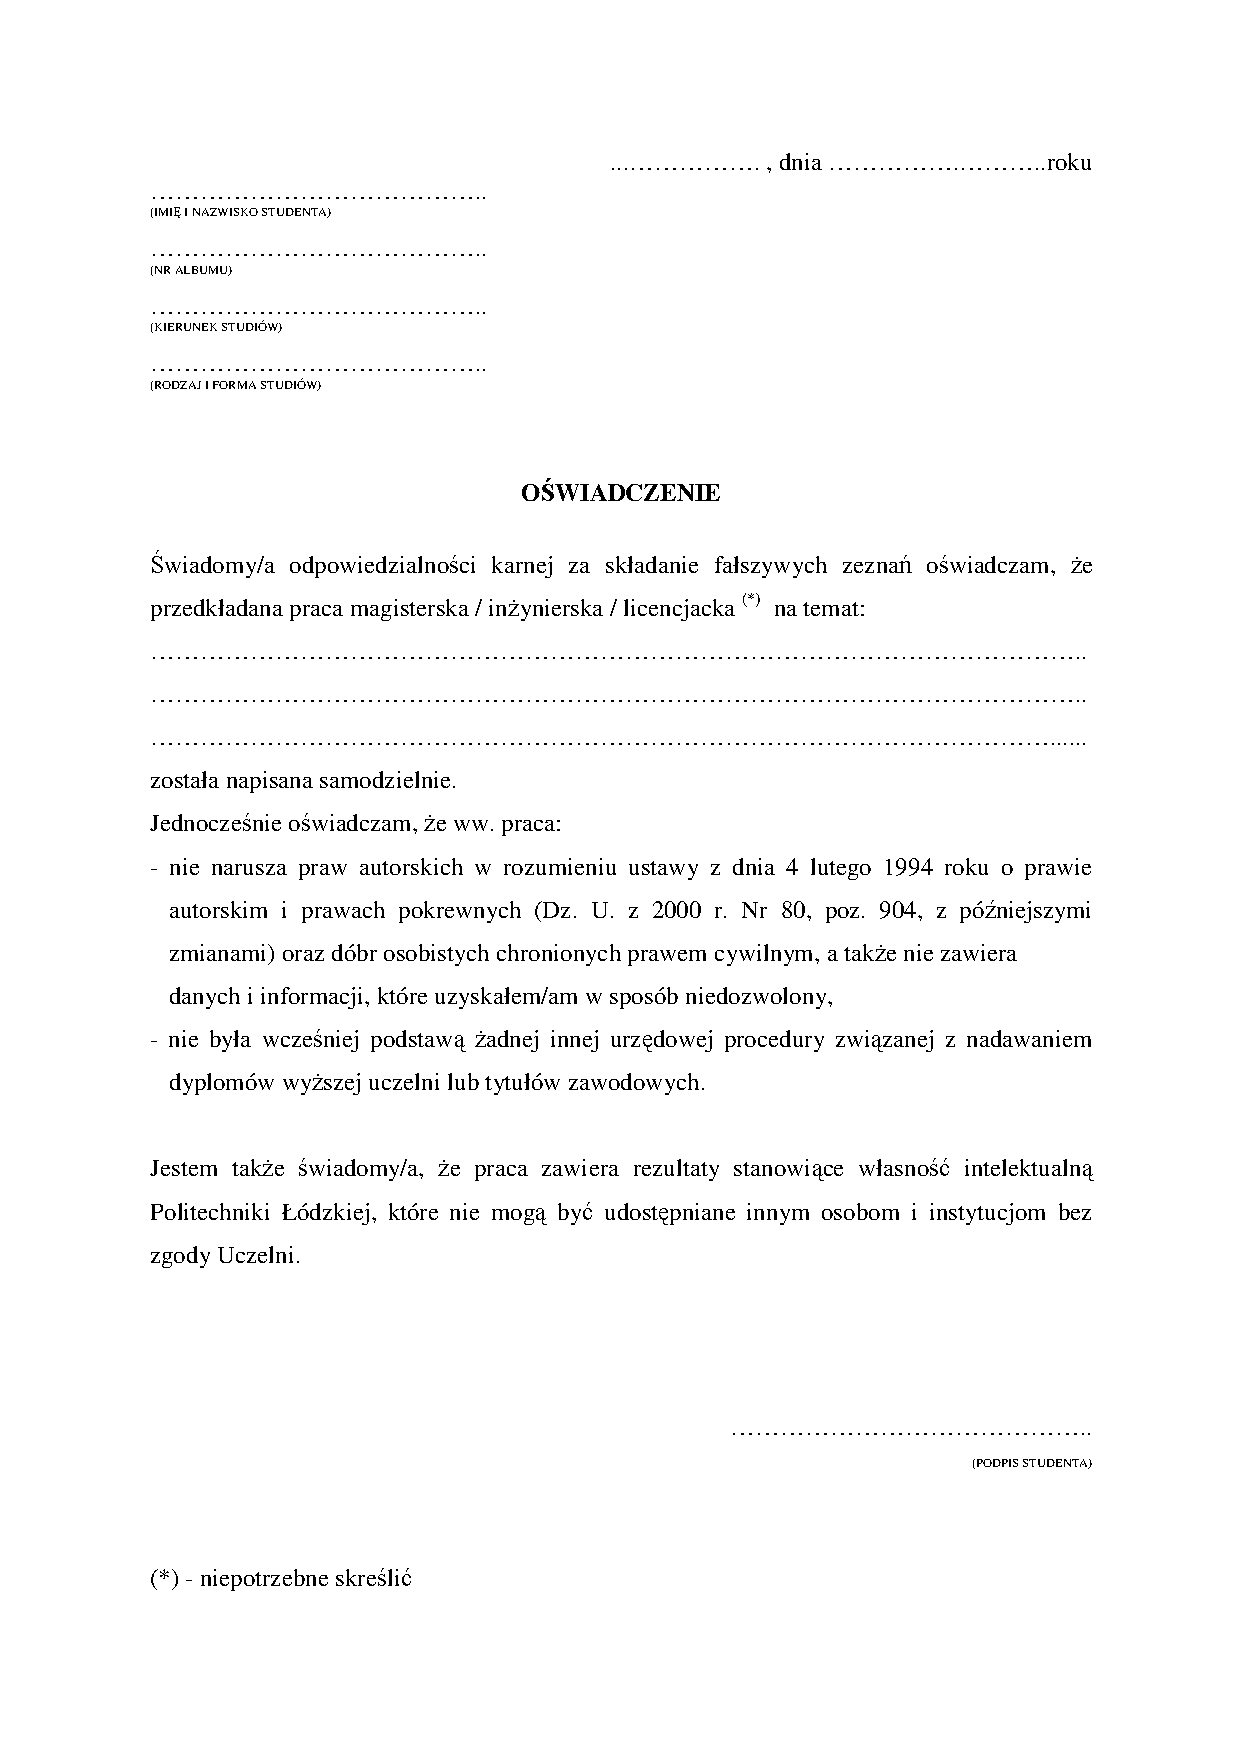
\includegraphics{figures/oswiadczenie_o_samodzielnosci.pdf}
\end{textblock}

\end{document}
